\documentclass[12pt,a4paper]{article}

% ---------- Idioma y codificación ----------
\usepackage[utf8]{inputenc}
\usepackage[T1]{fontenc}
\usepackage{mathpazo}
% Si tu distribución no tiene instalado el idioma español, esta línea evita
% que la compilación falle (instalá "babel-spanish" para tenerlo completo).
\IfFileExists{spanish.ldf}
  {\usepackage[spanish,es-nodecimaldot,es-noshorthands]{babel}}
  {\usepackage[english]{babel}}
% Nota: la opción es-noshorthands (arriba) desactiva los shorthands "<" y ">"
% de babel-spanish, que de otro modo rompen la sintaxis de flechas de TikZ
% (">={...}").

% ---------- Página ----------
\usepackage[a4paper,top=3cm,bottom=2.5cm,left=2.5cm,right=2.5cm,headheight=1.5cm,headsep=0.8cm]{geometry}

% ---------- Utilidades ----------
\usepackage{graphicx}
\usepackage{fancyhdr}
\usepackage{lastpage}          % necesario para \pageref{LastPage}
\usepackage{xcolor}
\usepackage{enumitem}
\usepackage{tikz}
\usetikzlibrary{positioning,shapes.geometric,arrows.meta,calc,fit,backgrounds}
\usepackage[hidelinks]{hyperref}
\usepackage{titlesec}
\usepackage{float}
\usepackage{pdflscape}         % páginas apaisadas (figura del sistema completo)
\usepackage{booktabs}
\usepackage{longtable}
\usepackage{amsmath}
\usepackage{amssymb}
\usepackage{listings}
\usepackage[numbers]{natbib}
\bibliographystyle{unsrtnat}
\newcommand{\sectionbreak}{\clearpage}

% ---------- Estilo para código Verilog ----------
\definecolor{codegray}{gray}{0.96}
\definecolor{codekw}{RGB}{0,90,160}
\definecolor{codecom}{RGB}{100,120,100}
\definecolor{codestr}{RGB}{160,60,60}
\definecolor{codenum}{gray}{0.45}

\lstdefinestyle{verilog}{
  language=Verilog,
  backgroundcolor=\color{codegray},
  basicstyle=\ttfamily\scriptsize,
  keywordstyle=\color{codekw}\bfseries,
  commentstyle=\color{codecom}\itshape,
  stringstyle=\color{codestr},
  numbers=left,
  numberstyle=\tiny\color{codenum},
  numbersep=8pt,
  showstringspaces=false,
  breaklines=true,
  breakatwhitespace=true,
  frame=single,
  rulecolor=\color{gray!40},
  framesep=4pt,
  xleftmargin=16pt,
  tabsize=4,
  captionpos=b,
  columns=fullflexible,
  morekeywords={always,posedge,negedge,localparam,parameter,logic,endcase,
                signed,unsigned,task,endtask,function,endfunction,initial,
                integer,timescale,display,finish,random,time,clog2,signed}
}
\lstset{style=verilog}
\renewcommand{\lstlistingname}{Código}

% ============================================================
%  >>>>>>>>>>  DATOS DEL TRABAJO: EDITAR ACÁ  <<<<<<<<<<
% ============================================================
\newcommand{\Titulo}{Trabajo Práctico N°3: Pipeline de un Procesador}
\newcommand{\Subtitulo}{}
\newcommand{\Materia}{Arquitectura de Computadoras}
\newcommand{\Institucion}{Facultad de Ciencias Exactas, Físicas y Naturales - Universidad Nacional de Córdoba}
\newcommand{\Carrera}{Ingeniería en Computación}
%\newcommand{\Fecha}{\today}

% Integrantes: una línea \persona{...} por cada uno
\newcommand{\Integrantes}{%
  \persona{Brigido, Tomás Andrés}{Legajo 38481096}%
  \persona{Tosolini, Agustín}{Legajo 42332698}%
}

% Docentes
\newcommand{\Docentes}{%
  \persona{Pereyra, Martin}{}%
}

% Repositorio: dejar vacío {} para que NO aparezca en la carátula
\newcommand{\Repositorio}{https://github.com/Agustin-Tosolini/Computer-Architecture-FCEFyN/tree/main/Laboratories/Lab3}

% Logos del encabezado
\newcommand{\LogoIzquierdo}{./logos/unc.png}
\newcommand{\LogoDerecho}{./logos/fcefyn.png}
\newcommand{\AlturaLogo}{3.0cm}
% ============================================================


% ---------- Maquinaria interna (no hace falta tocar) ----------
\newcommand{\ponerlogo}[1]{%
  \IfFileExists{#1}{%
    \includegraphics[height=\AlturaLogo,keepaspectratio]{#1}%
  }{%
    
\begin{tikzpicture}
      \node[draw=gray!60,dashed,fill=gray!10,rounded corners,
            minimum height=\AlturaLogo,minimum width=2.6cm,
            font=\scriptsize\color{gray}] {logo};
    \end{tikzpicture}%
  }%
}

% Imagen pendiente: si el archivo existe lo incluye, si no dibuja un recuadro
% punteado con el nombre esperado. Uso: \imagenpendiente{ancho}{archivo}
\newcommand{\imagenpendiente}[2]{%
  \IfFileExists{#2}{%
    \includegraphics[width=#1]{#2}%
  }{%
    \begin{tikzpicture}
      \node[draw=gray!60,dashed,fill=gray!10,rounded corners,
            minimum height=5cm,minimum width=#1,align=center,
            font=\small\color{gray}] {Imagen pendiente\\[2pt]\texttt{\detokenize{#2}}};
    \end{tikzpicture}%
  }%
}

% Estilo de la carátula: sin encabezado (los logos van dentro de la página)
\fancypagestyle{caratula}{%
  \fancyhf{}
  \renewcommand{\headrulewidth}{0pt}
  \renewcommand{\footrulewidth}{0pt}
}

% Resto del documento: sólo el número de página al pie, SIN logos
\fancypagestyle{plain}{%
  \fancyhf{}
  \fancyfoot[C]{\small Página \thepage\ de \pageref{LastPage}}
  \renewcommand{\headrulewidth}{0pt}
  \renewcommand{\footrulewidth}{0pt}
}
\pagestyle{plain}

\newcommand{\persona}[2]{%
  \textbf{#1}%
  \ifx\relax#2\relax\else{\ \small(#2)}\fi\\[0.25em]
}

\setlength{\emergencystretch}{3em}
\hyphenpenalty=1000
\setlength{\parskip}{0.6em}
\setlength{\parindent}{0pt}

% ---------- Imágenes, datos pendientes y comandos ----------
\graphicspath{{img/}}
% Dato que solo se obtiene de Vivado o de la placa: se marca en rojo para
% completarlo (no se inventa).
\newcommand{\completar}[1]{\textcolor{red}{\textbf{[COMPLETAR: #1]}}}
% Comando del protocolo de la Debug Unit (un byte ASCII)
\newcommand{\cmd}[1]{\textbf{\texttt{#1}}}
\usepackage{caption}
\captionsetup{font=small,labelfont=bf}
\usepackage{array}
\newcolumntype{L}[1]{>{\raggedright\arraybackslash}p{#1}}

% ---------- Estilos de TikZ para los diagramas ----------
\tikzset{
  bloque/.style   = {draw, rounded corners, align=center, font=\small,
                     minimum width=2.8cm, minimum height=1.3cm},
  estado/.style   = {draw, rounded corners, align=center, font=\small,
                     minimum width=3.2cm, minimum height=0.9cm},
  salida/.style   = {draw, rounded corners, align=center, font=\small,
                     minimum width=3.2cm, minimum height=1.3cm},
  etiqueta/.style = {font=\scriptsize, align=left},
  flecha/.style   = {-{Stealth[length=2mm]}}
}


% ============================================================
\begin{document}

% ------------------------- CARÁTULA -------------------------
\thispagestyle{caratula}
\begin{center}
  % --- Logos: aparecen únicamente en esta página
  \noindent\makebox[\textwidth]{%
    \ponerlogo{\LogoIzquierdo}\hfill\ponerlogo{\LogoDerecho}%
  }\\[0.35cm]
  \rule{\textwidth}{0.4pt}

  \vspace{0.5cm}

  {\large \Institucion \par}
  {\normalsize \Carrera \par}

  \vspace{0.5cm}
  \rule{\textwidth}{1.2pt}\\[0.6cm]
  {\Huge\bfseries \Titulo \par}
  \vspace{0.3cm}
  \ifx\Subtitulo\empty\else{\Large \Subtitulo \par}\vspace{0.3cm}\fi
  \rule{\textwidth}{1.2pt}

  \vspace{0.7cm}
  {\large \textit{\Materia} \par}

  \vspace{0.75cm}
  {\large\bfseries Integrantes\par}
  \vspace{0.4cm}
  \Integrantes

  \vspace{1cm}
  {\large\bfseries Docente\par}
  \vspace{0.4cm}
  \Docentes

  \vspace{1cm}
  {\large\bfseries Repositorio\par}
  \vspace{0.4cm}
  \Repositorio

  \vfill

  %{\large \Fecha \par}
  \vspace{1cm}
\end{center}

\newpage

% --------------------- ÍNDICE ---------------------
\tableofcontents
\newpage



% ============================================================
\section{Introducción}
% ============================================================

El objetivo del trabajo es implementar en una FPGA (placa Digilent Basys~3,
Artix-7 XC7A35T) un procesador RISC-V de 32~bits con \textbf{pipeline de cinco
etapas}, junto con una \textbf{Debug Unit} que permite programarlo, ejecutarlo y
observar su estado completo desde una PC a través de la UART, y un
\textbf{software de PC} para escribir programas en ensamblador e interactuar con
el sistema.

La consigna pide:
\begin{itemize}[nosep]
  \item el pipeline IF, ID, EX, MEM, WB con las instrucciones de RV32I
        indicadas, resolviendo los riesgos estructurales, de datos y de control;
  \item enviar a la PC, por UART, los 32 registros, los latches intermedios y la
        memoria de datos usada;
  \item cargar y recargar el programa por UART, sin resintetizar, a partir de
        un programa escrito en ensamblador con una instrucción de parada;
  \item dos modos de operación: \emph{continuo} y \emph{paso a paso} (un ciclo
        de clock por comando), con el pipeline vacío al terminar;
  \item no intervenir el clock en ninguna parte del diseño, y analizar el camino
        crítico, el skew y la frecuencia de funcionamiento.
\end{itemize}

El trabajo se organizó en tres partes que se conectan mediante un
\emph{contrato} escrito de antemano (\texttt{src/params.vh}):

\begin{description}[nosep,leftmargin=1.2cm,style=nextline]
  \item[Parte A] el procesador (\texttt{src/cpu/}).
  \item[Parte B] la comunicación UART y la Debug Unit (\texttt{src/debug\_unit/}).
  \item[Parte C] el software de PC en Python (\texttt{scripts/}): ensamblador,
        modelo de referencia, herramienta de consola y depurador gráfico.
\end{description}

El resultado es un sistema completo y verificado: el RTL compila sin warnings
con Icarus Verilog (\texttt{-Wall -g2005}), todos los testbenches son
autoverificados y dan PASS, y el comportamiento del hardware coincide ciclo a
ciclo con un modelo de referencia independiente. El diseño final funciona a
62,5~MHz en la placa. La figura~\ref{fig:sistema}, en la página siguiente,
muestra el sistema completo.

\begin{landscape}
\begin{figure}[p]
  \centering
  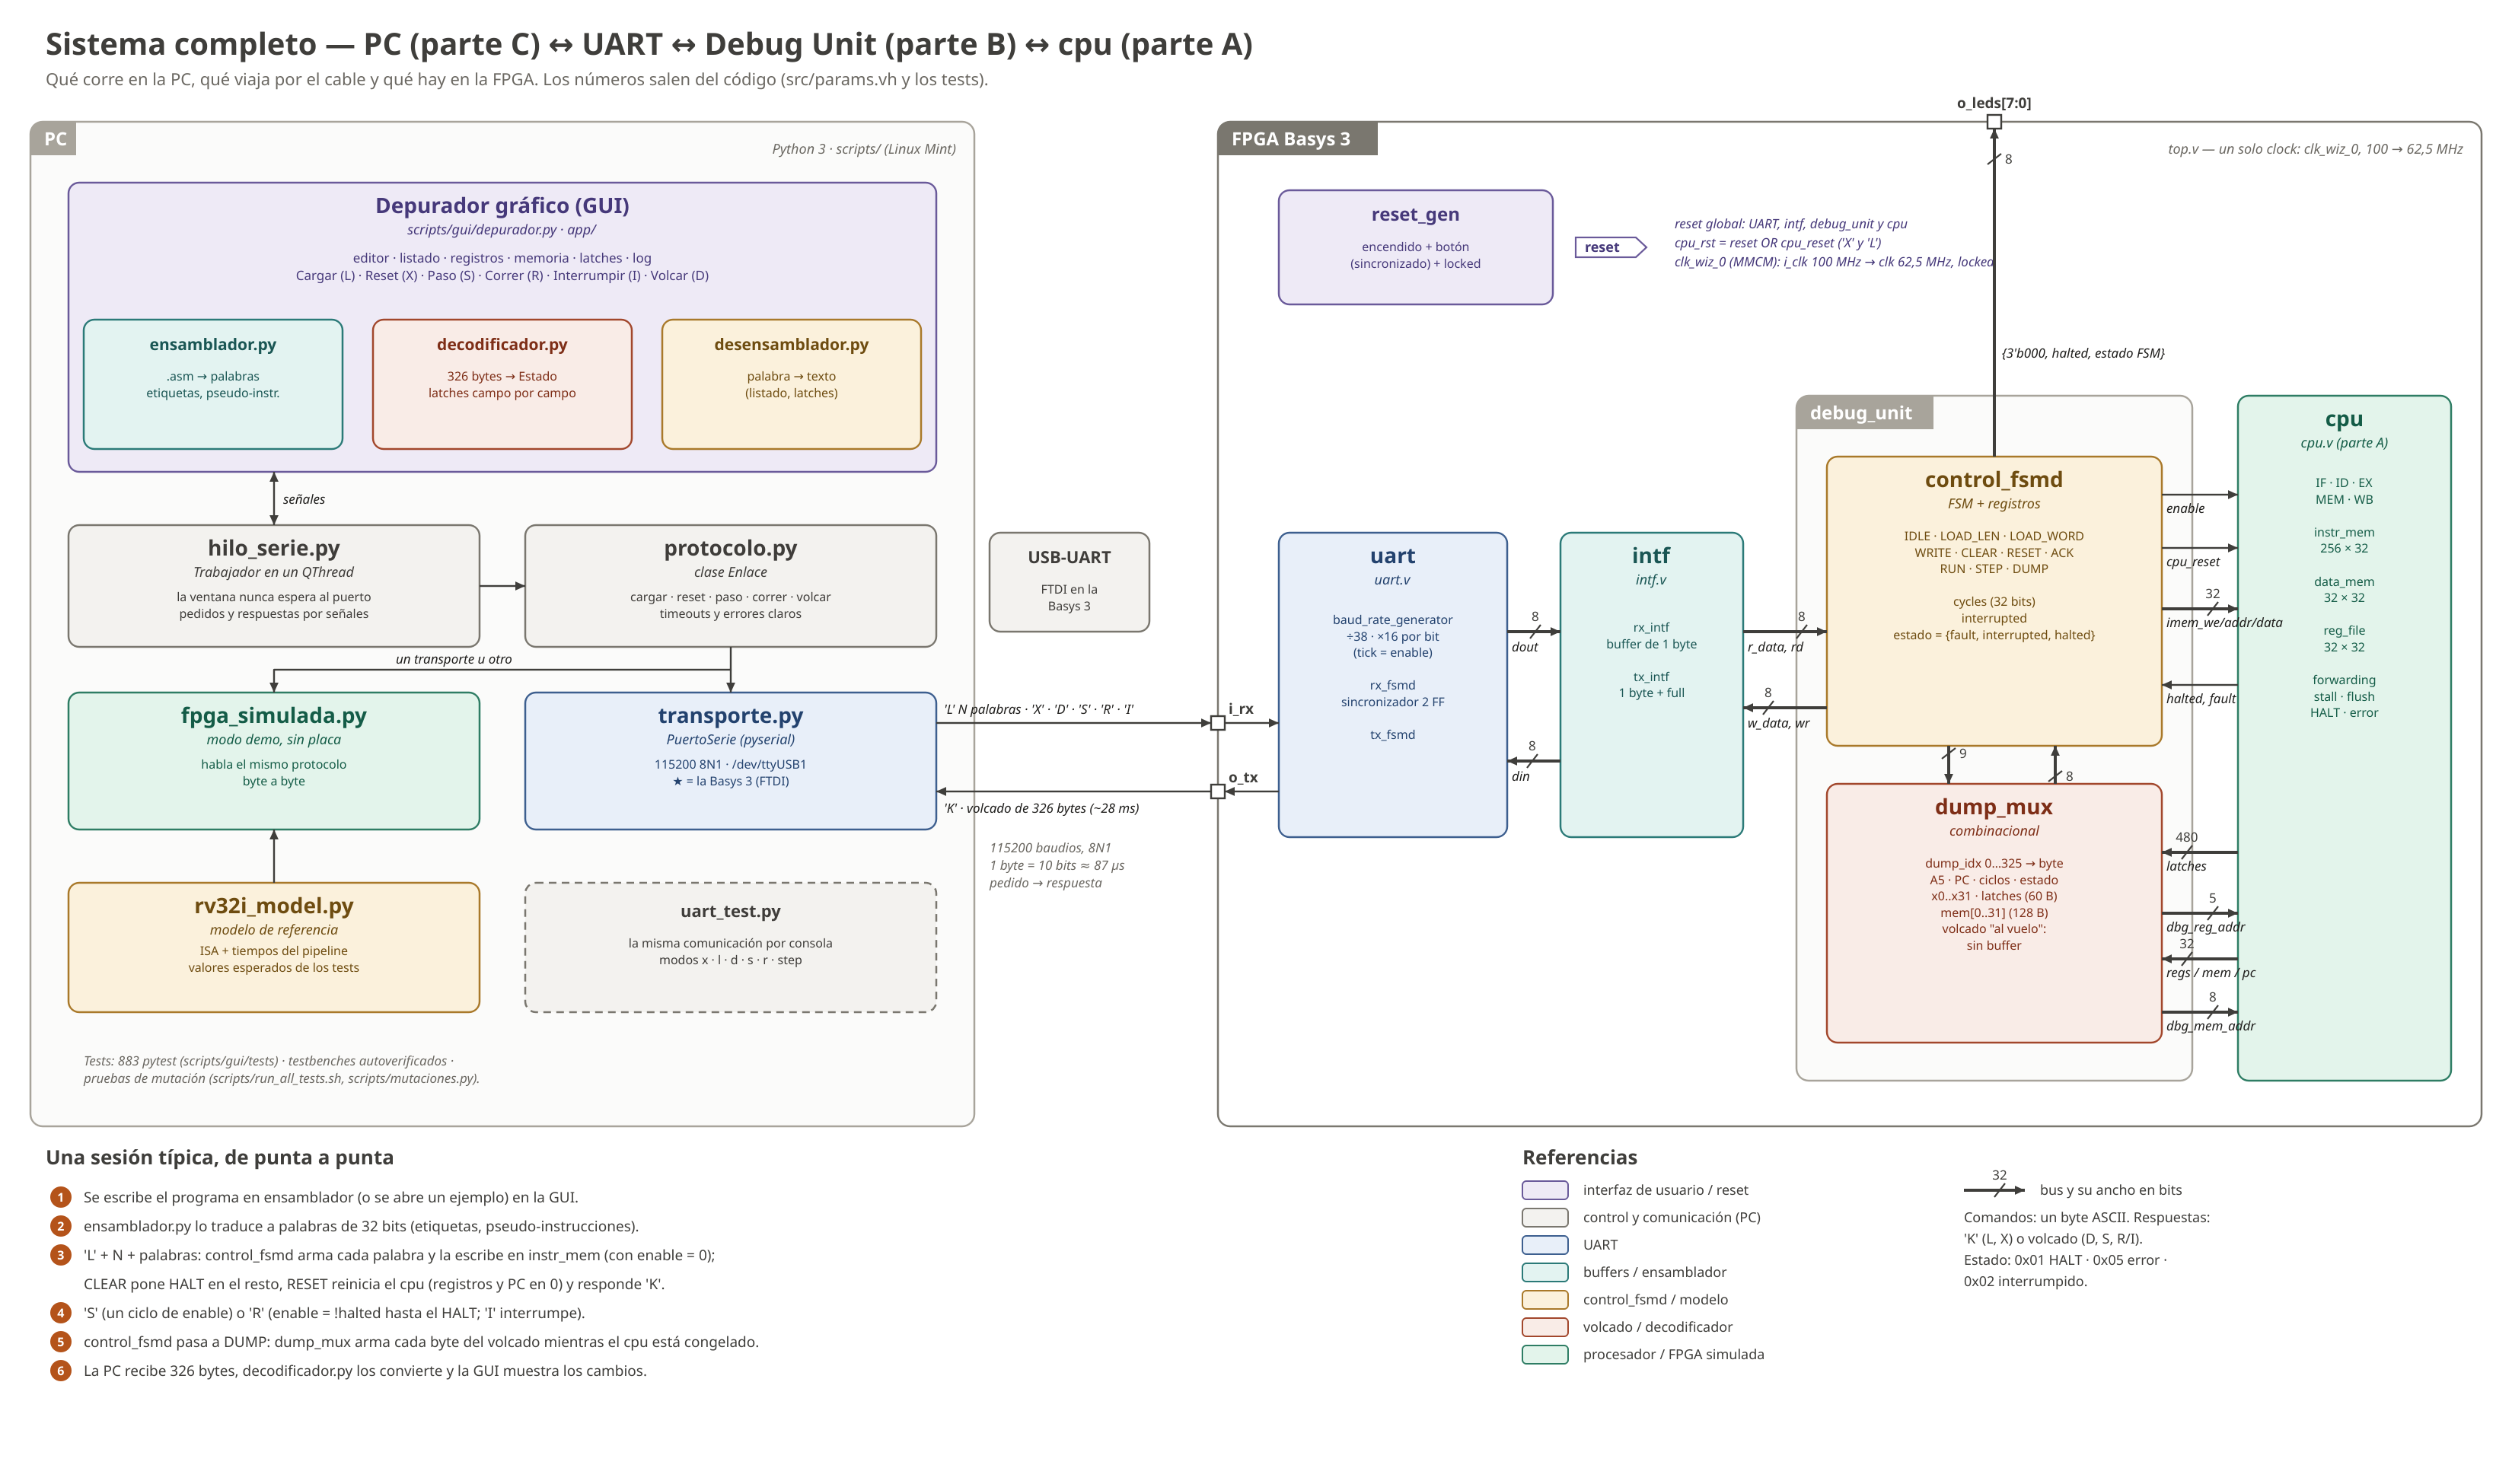
\includegraphics[width=\linewidth,height=0.9\textheight,keepaspectratio]{sistema_completo.png}
  \caption{Sistema completo: software de PC (parte C), enlace UART, Debug Unit
  (parte B) y procesador (parte A), con la secuencia de una sesión típica.}
  \label{fig:sistema}
\end{figure}
\end{landscape}

% ============================================================
\section{Marco teórico}
% ============================================================

\subsection{La arquitectura RV32I}

RV32I es el conjunto base de instrucciones enteras de RISC-V para 32~bits
\cite{riscv}: 32 registros de 32~bits (\texttt{x0} vale siempre cero),
instrucciones de 32~bits y memoria direccionada por byte. Las instrucciones se
codifican en seis formatos (R, I, S, B, U, J) que comparten una propiedad
importante para el hardware: \textbf{los campos de registro están siempre en la
misma posición} (\texttt{rs1} en los bits 19:15, \texttt{rs2} en 24:20,
\texttt{rd} en 11:7) y el bit~31 es siempre el signo del inmediato. Así, el
banco de registros puede leerse en paralelo con la decodificación y la
extensión de signo no depende del formato. Los inmediatos de los saltos (B y J)
no guardan el bit~0, que siempre vale cero, lo que duplica el alcance con el
mismo campo.

Se implementaron las 32 instrucciones de la consigna:

\begin{table}[H]
\centering
\small
\begin{tabular}{@{}lL{10.5cm}@{}}
\toprule
Tipo & Instrucciones \\
\midrule
R & \texttt{add sub sll srl sra and or xor slt sltu} \\
I aritméticas & \texttt{addi andi ori xori slti sltiu slli srli srai} \\
I cargas & \texttt{lb lh lw lbu lhu} \\
I salto & \texttt{jalr} \\
S & \texttt{sb sh sw} \\
B & \texttt{beq bne} \\
U & \texttt{lui} \\
J & \texttt{jal} \\
Propia & \texttt{HALT} = \texttt{0x00000000} \\
\bottomrule
\end{tabular}
\caption{Instrucciones implementadas.}
\end{table}

\subsection{Pipeline de cinco etapas}

En un procesador monociclo cada instrucción recorre todo el camino de datos en
un único ciclo, cuyo período lo fija la instrucción más lenta. El
\emph{pipeline} divide ese camino en etapas separadas por registros, de modo que
cada etapa trabaja sobre una instrucción distinta \cite{patterson}:

\begin{description}[nosep,leftmargin=1.5cm,style=sameline]
  \item[IF] busca la instrucción en la dirección del PC.
  \item[ID] decodifica, lee los registros y arma el inmediato.
  \item[EX] opera en la ALU y resuelve los saltos.
  \item[MEM] lee o escribe la memoria de datos.
  \item[WB] escribe el resultado en el registro destino.
\end{description}

Cada instrucción tarda cinco ciclos (latencia), pero en régimen termina una por
ciclo (throughput), con un período más corto. El CPI ideal es 1; en la práctica
es mayor por los \emph{riesgos}:

\begin{itemize}[nosep]
  \item \textbf{Estructurales:} dos instrucciones necesitan el mismo recurso en
        el mismo ciclo.
  \item \textbf{De datos:} una instrucción necesita un resultado que todavía no
        se escribió en el banco de registros. Se resuelven con
        \emph{forwarding} (tomar el dato de los registros de pipeline) y, cuando
        no alcanza (load-use), con un \emph{stall}.
  \item \textbf{De control:} no se sabe cuál es la instrucción siguiente hasta
        resolver un salto. Las instrucciones buscadas de más se descartan
        (\emph{flush}).
\end{itemize}

\subsection{Control de la ejecución sin intervenir el clock}

Para pausar un circuito sincrónico hay dos alternativas. El \emph{clock gating}
(cortar el clock con lógica) está prohibido por la consigna y es una mala
práctica en FPGA: el clock deja la red de distribución dedicada, aparecen
glitches y skew, y se invalida el análisis de timing. La alternativa correcta es
el \textbf{clock enable}: el clock llega siempre a todos los flip-flops y cada
uno tiene una habilitación; con la habilitación en cero conserva su valor. Las
FPGA de Xilinx tienen esa entrada en el propio flip-flop, sin costo adicional.

\subsection{Comunicación UART}

La UART es una comunicación serie asincrónica: cada extremo usa su propio
clock y ambos acuerdan la velocidad. El formato 8N1 transmite un bit de start
(0), ocho bits de datos empezando por el menos significativo, sin paridad, y un
bit de stop (1). El receptor \emph{sobremuestrea} la línea 16~veces por bit:
detecta el flanco del start, se ubica en el centro del bit y muestrea cada bit
en su centro, lo que tolera diferencias de velocidad entre los dos lados
\cite{chu}. Como la línea de recepción es asincrónica respecto del clock de la
FPGA, debe pasar por un sincronizador de dos flip-flops para evitar que la
metaestabilidad llegue a la lógica.

\subsection{Timing}

Para que el diseño funcione, cada camino combinacional entre dos flip-flops debe
terminar antes del flanco siguiente, respetando el tiempo de \emph{setup}, y no
puede cambiar la entrada demasiado pronto después del flanco (tiempo de
\emph{hold}). El \emph{slack} es el margen que queda; el WNS (\emph{Worst
Negative Slack}) es el peor slack de setup del diseño: si es mayor o igual a
cero, el diseño cumple a esa frecuencia. El camino con menos slack es el
\emph{camino crítico} y fija la frecuencia máxima,
$f_{\max} \approx 1/(T - \text{WNS})$. El \emph{skew} es la diferencia en el
instante de llegada del clock a distintos flip-flops; en la FPGA se mantiene
bajo distribuyendo el clock por la red global dedicada. Para generar una
frecuencia distinta de la del oscilador se usa un MMCM (\emph{Clocking
Wizard}), con $f_{\text{VCO}} = f_{\text{in}} \cdot M / D$ y
$f_{\text{out}} = f_{\text{VCO}} / O$; su salida \texttt{locked} indica que el
clock generado es estable \cite{ug472,pg065}.

% ============================================================
\section{Arquitectura del sistema}
% ============================================================

\subsection{Contrato entre el procesador y la Debug Unit}

Para que las partes A y B pudieran desarrollarse en paralelo, primero se fijó
la interfaz entre ellas en \texttt{src/params.vh}: nombres, anchos y
comportamiento de cada señal, el protocolo y el formato del volcado. El archivo
es solo documentación (ningún módulo lo incluye), pero los tests verifican que
el RTL y el software coincidan con él. Mientras el procesador no estaba listo,
la Debug Unit se desarrolló y probó en la placa contra un \texttt{cpu\_stub}:
un procesador falso con exactamente los mismos puertos.

\begin{table}[H]
\centering
\small
\begin{tabular}{@{}L{5.2cm}lL{7.4cm}@{}}
\toprule
Señal & Ancho & Semántica \\
\midrule
\texttt{i\_clk} & 1 & clock del sistema, nunca intervenido \\
\texttt{i\_enable} & 1 & clock enable: con 1 avanza un ciclo por flanco; con 0 todo queda congelado \\
\texttt{i\_cpu\_reset} & 1 & pulso sincrónico: PC, latches, registros, \texttt{halted} y \texttt{fault} en cero; no borra las memorias \\
\texttt{i\_imem\_we/addr/data} & 1/8/32 & escritura de la memoria de programa, solo con \texttt{i\_enable} = 0 \\
\texttt{i\_dbg\_reg\_addr} $\rightarrow$ \texttt{o\_dbg\_reg\_data} & 5 $\rightarrow$ 32 & lectura asincrónica de un registro (\texttt{x0} = 0) \\
\texttt{i\_dbg\_mem\_addr} $\rightarrow$ \texttt{o\_dbg\_mem\_data} & 8 $\rightarrow$ 32 & lectura asincrónica de una palabra de la memoria de datos \\
\texttt{o\_pc} & 32 & PC de búsqueda (en bytes) \\
\texttt{o\_latches} & 480 & los cuatro registros de pipeline concatenados \\
\texttt{o\_halted} & 1 & el HALT llegó a WB; queda en 1 hasta el reset \\
\texttt{o\_fault} & 1 & la parada fue por error (junto con \texttt{o\_halted}) \\
\bottomrule
\end{tabular}
\caption{Interfaz entre el procesador y la Debug Unit (\texttt{params.vh}, sección~4).}
\end{table}

\subsection{Procesador (parte A)}

\begin{figure}[H]
  \centering
  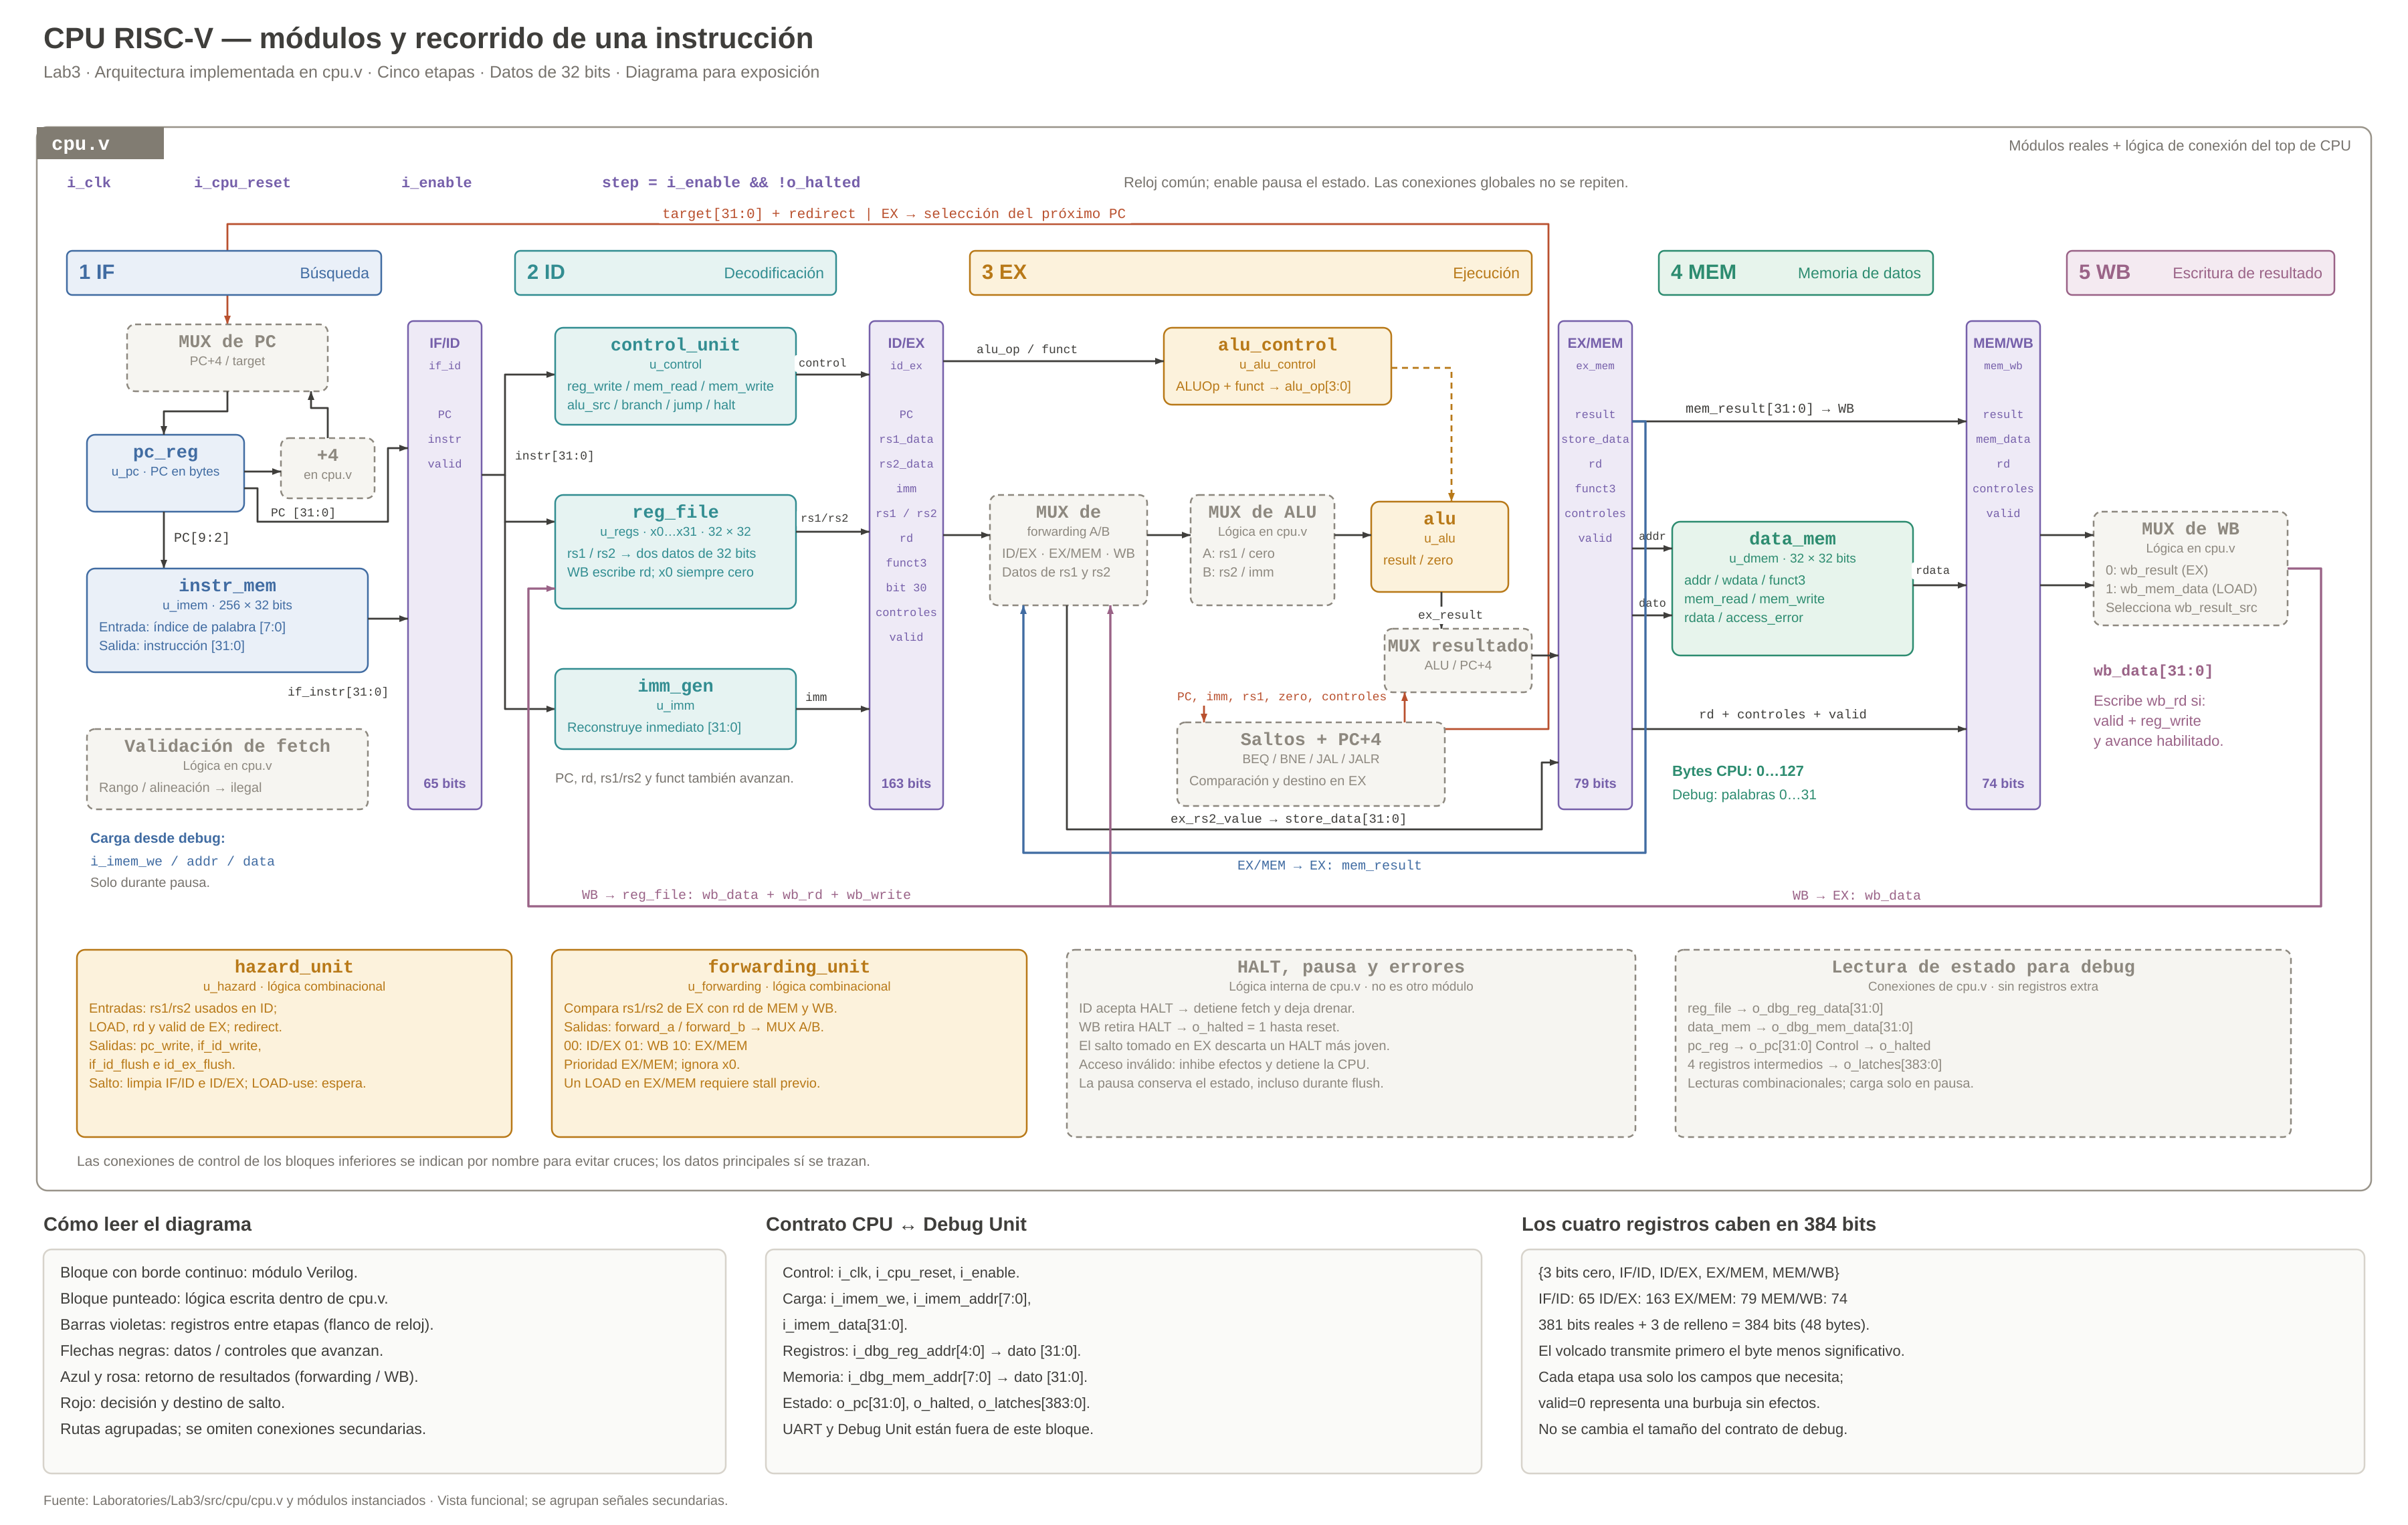
\includegraphics[width=\textwidth]{CPU_completo.png}
  \caption{Camino de datos del procesador: etapas, registros de pipeline,
  forwarding (azul), escritura en WB (violeta) y saltos (rojo).}
  \label{fig:cpu}
\end{figure}

La figura~\ref{fig:cpu} muestra el procesador (\texttt{src/cpu/cpu.v}). Los
módulos se agrupan por etapa: \texttt{pc\_reg} e \texttt{instr\_mem} (IF);
\texttt{control\_unit}, \texttt{reg\_file} e \texttt{imm\_gen} (ID);
\texttt{alu\_control} y \texttt{alu} (EX); \texttt{data\_mem} (MEM); los cuatro
registros de pipeline (\texttt{if\_id}, \texttt{id\_ex}, \texttt{ex\_mem},
\texttt{mem\_wb}); y las unidades \texttt{forwarding\_unit} y
\texttt{hazard\_unit}. Los multiplexores, el sumador del PC y la lógica de
saltos y de parada están en \texttt{cpu.v}.

\subsubsection{Memorias y banco de registros}

\begin{itemize}[nosep]
  \item \textbf{Memoria de programa:} 256 palabras de 32~bits (1~KiB), RAM
        distribuida con lectura asincrónica. IF lee la instrucción en el mismo
        ciclo. No se borra con el reset.
  \item \textbf{Memoria de datos:} 32 palabras (128~bytes), RAM distribuida
        con lectura asincrónica y escritura por byte (\texttt{sb}, \texttt{sh}).
        Es exactamente lo que muestra el volcado, de modo que toda la memoria
        es visible. Un acceso fuera de 0..127 o desalineado detiene el
        procesador con error. No se borra con el reset.
  \item \textbf{Banco de registros:} 32 registros de 32~bits en flip-flops,
        con dos lecturas para ID, una escritura en WB, reset y un
        \emph{bypass} WB $\rightarrow$ ID: si en un ciclo WB escribe el registro
        que ID está leyendo, el banco entrega el dato nuevo.
\end{itemize}

Se eligió RAM distribuida y no Block RAM porque esta última tiene lectura
sincrónica: obligaría a agregar un ciclo de latencia en IF y en MEM y a
reformular los stalls. Con memorias chicas la RAM distribuida es suficiente, y
permite además que la Debug Unit arme el volcado leyendo la memoria en el mismo
ciclo.

\subsubsection{Registros de pipeline}

Los registros entre etapas (llamados \emph{latches} en la consigna, aunque son
flip-flops por flanco) guardan los datos y las señales de control que la
instrucción necesita en las etapas siguientes. Las señales de control se
``gastan'': ID/EX lleva las de EX, MEM y WB; EX/MEM ya no lleva las de la ALU; y
MEM/WB solo las de WB. Cada registro tiene un bit \texttt{valid}: una
\emph{burbuja} es una instrucción con \texttt{valid} = 0 que no produce efectos
(IF/ID guarda la instrucción NOP, nunca \texttt{0x00000000}, que sería HALT).
Los bits \texttt{halt} e \texttt{illegal} llevan hasta WB el marcador de
parada.

\begin{table}[H]
\centering
\small
\begin{tabular}{@{}lL{7.4cm}rr@{}}
\toprule
Registro & Campos & Bits & En el volcado \\
\midrule
IF/ID & pc, instr, valid & 65 & 96 \\
ID/EX & pc, rs1\_data, rs2\_data, imm, rs1, rs2, rd, funct3, bit~30, 16 controles, halt, illegal, valid & 163 & 192 \\
EX/MEM & result, store\_data, rd, funct3, controles de MEM y WB, halt, illegal, valid & 79 & 96 \\
MEM/WB & result, mem\_data, rd, reg\_write, result\_src, halt, illegal, valid & 74 & 96 \\
\midrule
Total & & 381 & 480 \\
\bottomrule
\end{tabular}
\caption{Registros de pipeline. En el volcado cada uno ocupa palabras enteras
de 32~bits (relleno en cero) para que cada dato se lea directamente en
hexadecimal; la tabla campo por campo está en \texttt{params.vh}, sección~4b.}
\end{table}

\subsubsection{Riesgos de datos: forwarding y load-use}

La \texttt{forwarding\_unit} compara los registros fuente de la instrucción en
EX con el destino de las instrucciones en EX/MEM y MEM/WB, y controla dos
multiplexores delante de la ALU. La condición completa es: la instrucción en EX
es válida y usa ese registro, la instrucción productora es válida y escribe un
registro, el \texttt{rd} coincide y es distinto de \texttt{x0}. Si ambas
coinciden, \textbf{EX/MEM tiene prioridad} por ser el resultado más reciente. El
forwarding alimenta los operandos de la ALU, el dato de los stores y la
comparación de los saltos. Un load en EX/MEM no se adelanta: su dato existe
recién al final de MEM.

Ese es el caso \emph{load-use}: si la instrucción siguiente a un load usa su
resultado, el forwarding no alcanza. La \texttt{hazard\_unit} lo detecta (load
válido en EX con \texttt{rd} $\neq 0$ usado por la instrucción en ID), congela el
PC e IF/ID e inserta una burbuja en ID/EX. Al ciclo siguiente el load está en WB
y el dato llega por forwarding MEM/WB. El costo es \textbf{exactamente un
ciclo}.

La figura~\ref{fig:fwd} muestra los dos caminos de forwarding en un mismo
ciclo, tal como los ve el depurador: \texttt{add x7, x6, x5} está en EX y toma
\texttt{x6} de EX/MEM (lo produjo la instrucción anterior) y \texttt{x5} de
MEM/WB (lo produjo la de dos antes), sin ningún stall.

\begin{figure}[H]
  \centering
  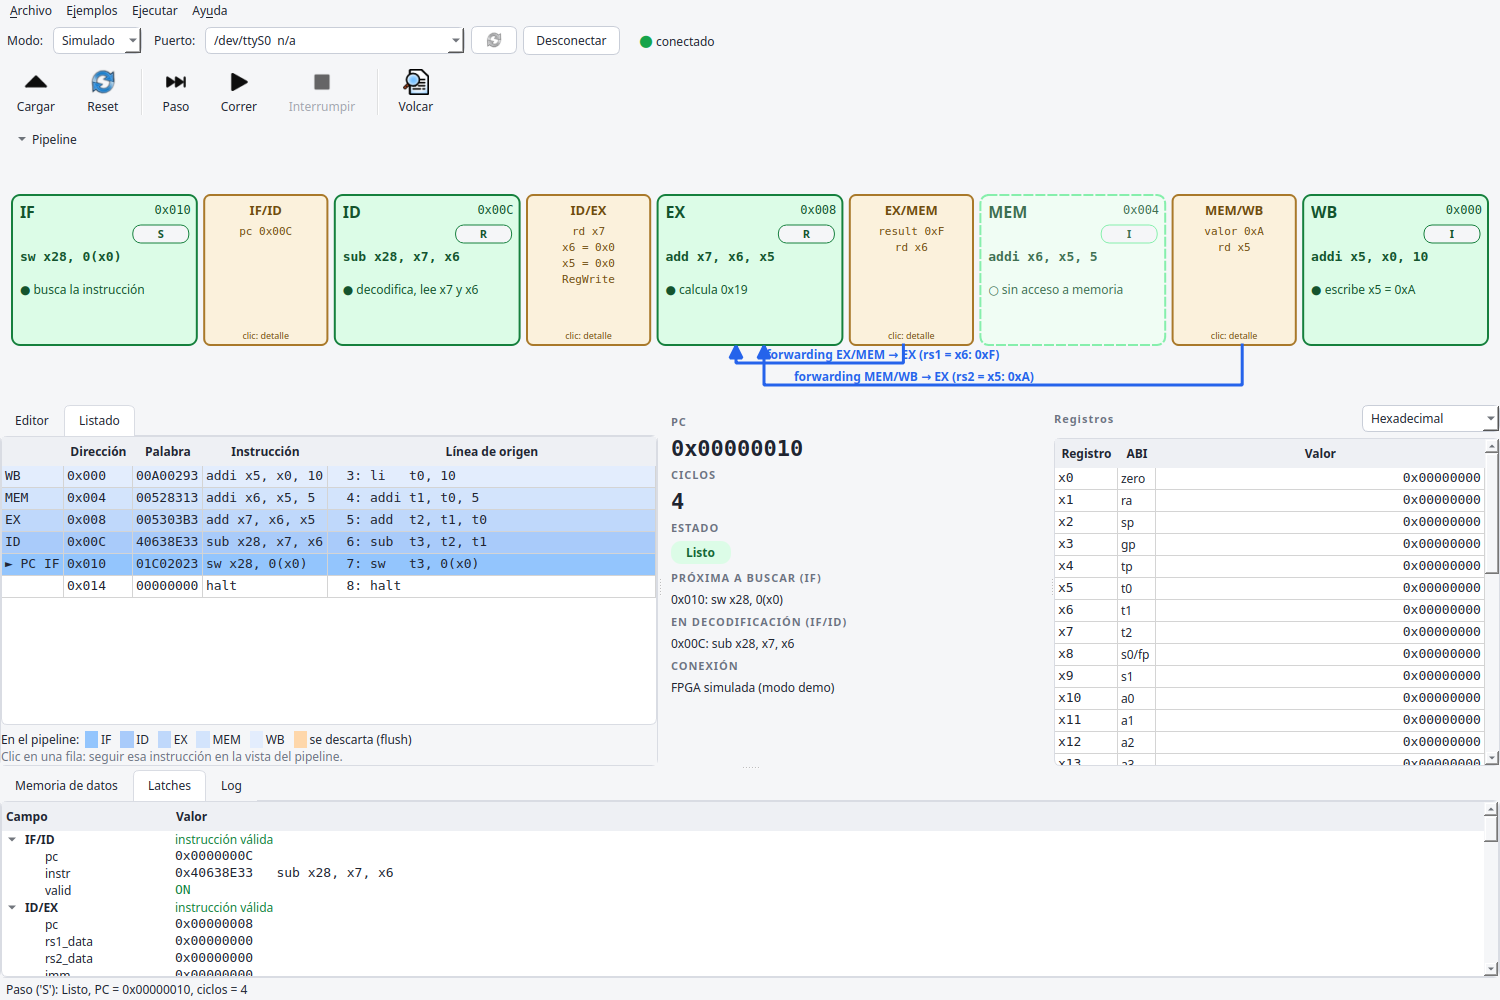
\includegraphics[width=\textwidth]{pipeline_forwarding.png}
  \caption{Forwarding EX/MEM $\rightarrow$ EX (\texttt{rs1 = x6}) y MEM/WB
  $\rightarrow$ EX (\texttt{rs2 = x5}) en el mismo ciclo, en el depurador.}
  \label{fig:fwd}
\end{figure}

\subsubsection{Riesgos de control: saltos}

Los saltos (\texttt{beq}, \texttt{bne}, \texttt{jal}, \texttt{jalr}) se
resuelven en EX, con los operandos ya corregidos por forwarding. Mientras tanto
IF sigue buscando en secuencia (equivale a predecir ``no tomado''). Si el salto
se toma, el PC toma el destino ---\texttt{PC + imm}, o
\texttt{(rs1 + imm) \& \textasciitilde 1} para \texttt{jalr}--- y se hace flush de
IF/ID e ID/EX: las dos instrucciones buscadas de más se convierten en burbujas.
Un salto tomado cuesta \textbf{2~ciclos}; uno no tomado, ninguno.
\texttt{jal} y \texttt{jalr} escriben \texttt{PC + 4} en \texttt{rd}. Resolver
el salto en ID habría bajado la penalidad a un ciclo, pero exige un comparador y
forwarding hacia ID y alarga una etapa que ya incluye la lectura del banco; se
priorizó un único mecanismo de forwarding en EX.

Con estas reglas, la cantidad de ciclos de un programa que termina es:
\[
  \text{ciclos} = N + 4 + \text{stalls} + 2 \cdot \text{saltos tomados},
\]
donde $N$ es la cantidad de instrucciones ejecutadas antes del HALT y el ``+4''
es el llenado y vaciado del pipeline.

\begin{figure}[H]
  \centering
  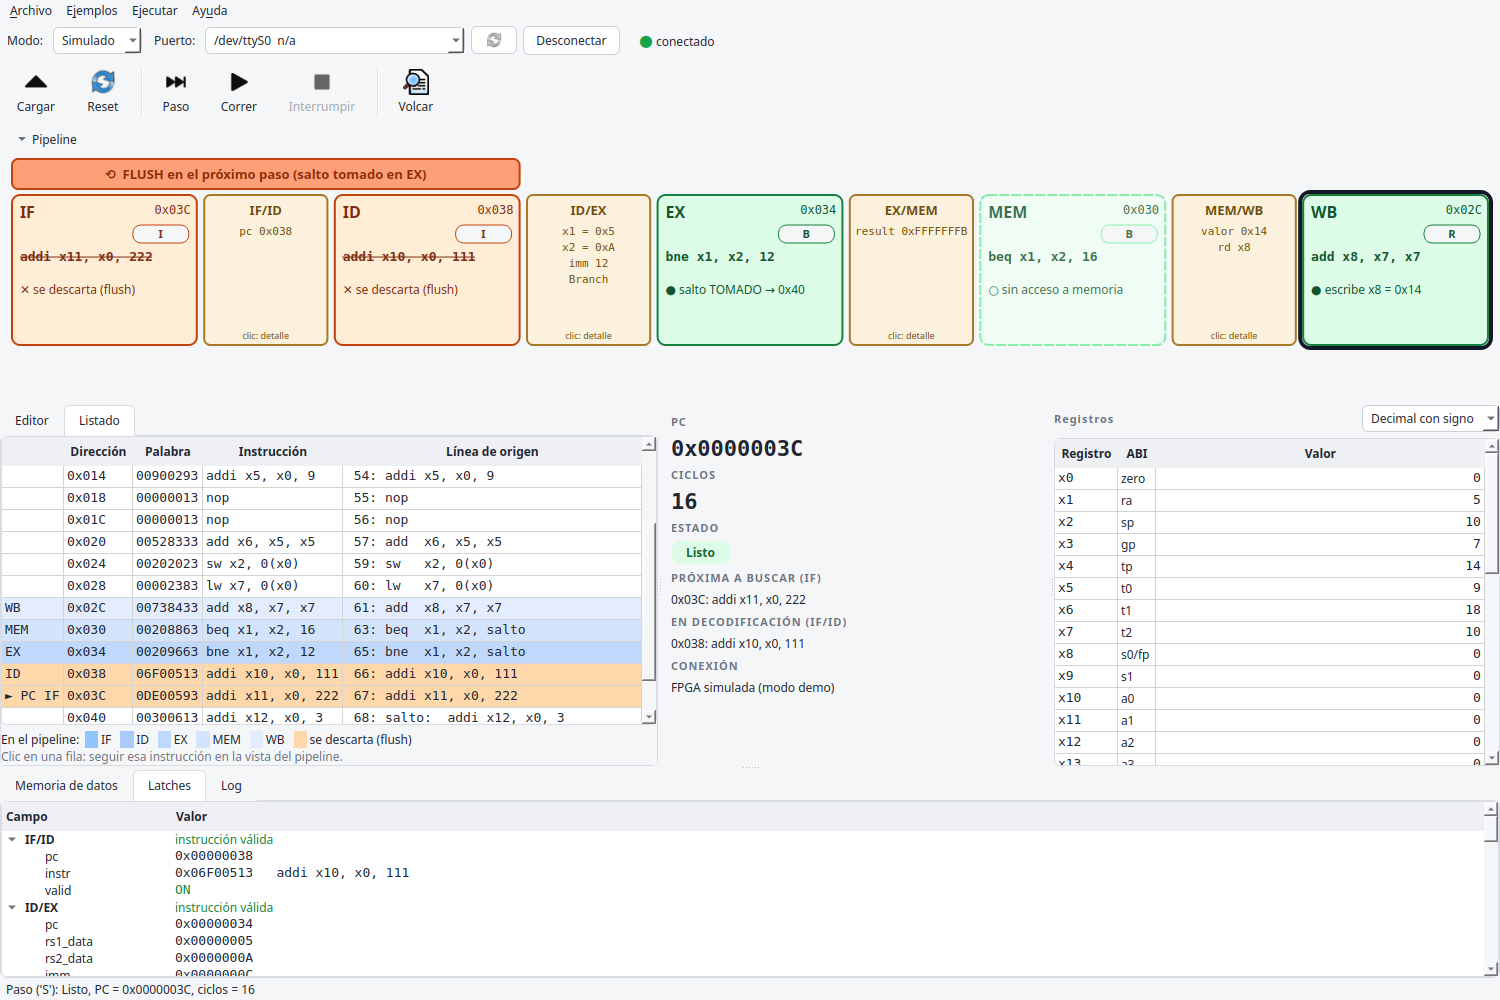
\includegraphics[width=\textwidth]{defensa_paso16_flush.png}
  \caption{Salto tomado: \texttt{bne x1, x2, 12} en EX se resuelve como tomado
  (destino 0x40) y las dos instrucciones buscadas de más, en IF e ID, se
  descartan en el próximo flanco (flush).}
  \label{fig:flush}
\end{figure}

\subsubsection{HALT, errores y pipeline vacío}

La instrucción de parada es \texttt{0x00000000}: no es una instrucción válida
de RISC-V, y una memoria vacía funciona como parada. El HALT se detecta en ID:
desde ese ciclo se deja de buscar (el PC queda congelado en la dirección del
HALT + 4) y el HALT baja como marcador sin escribir nada. La señal
\texttt{o\_halted = MEM/WB.valid $\land$ MEM/WB.halt} sube cuando el marcador
llega a WB: en ese flanco la última instrucción real ya escribió y las etapas
anteriores están vacías. Con cinco NOP seguidos de un HALT, \texttt{o\_halted}
vale 1 después de exactamente 9 ciclos. Un salto tomado en EX tiene prioridad
sobre un HALT más joven en ID, que queda en el camino descartado.
La figura~\ref{fig:halt} muestra el estado al terminar: el HALT en WB, las demás
etapas vacías y los registros de pipeline con \texttt{valid} = 0.

\begin{figure}[H]
  \centering
  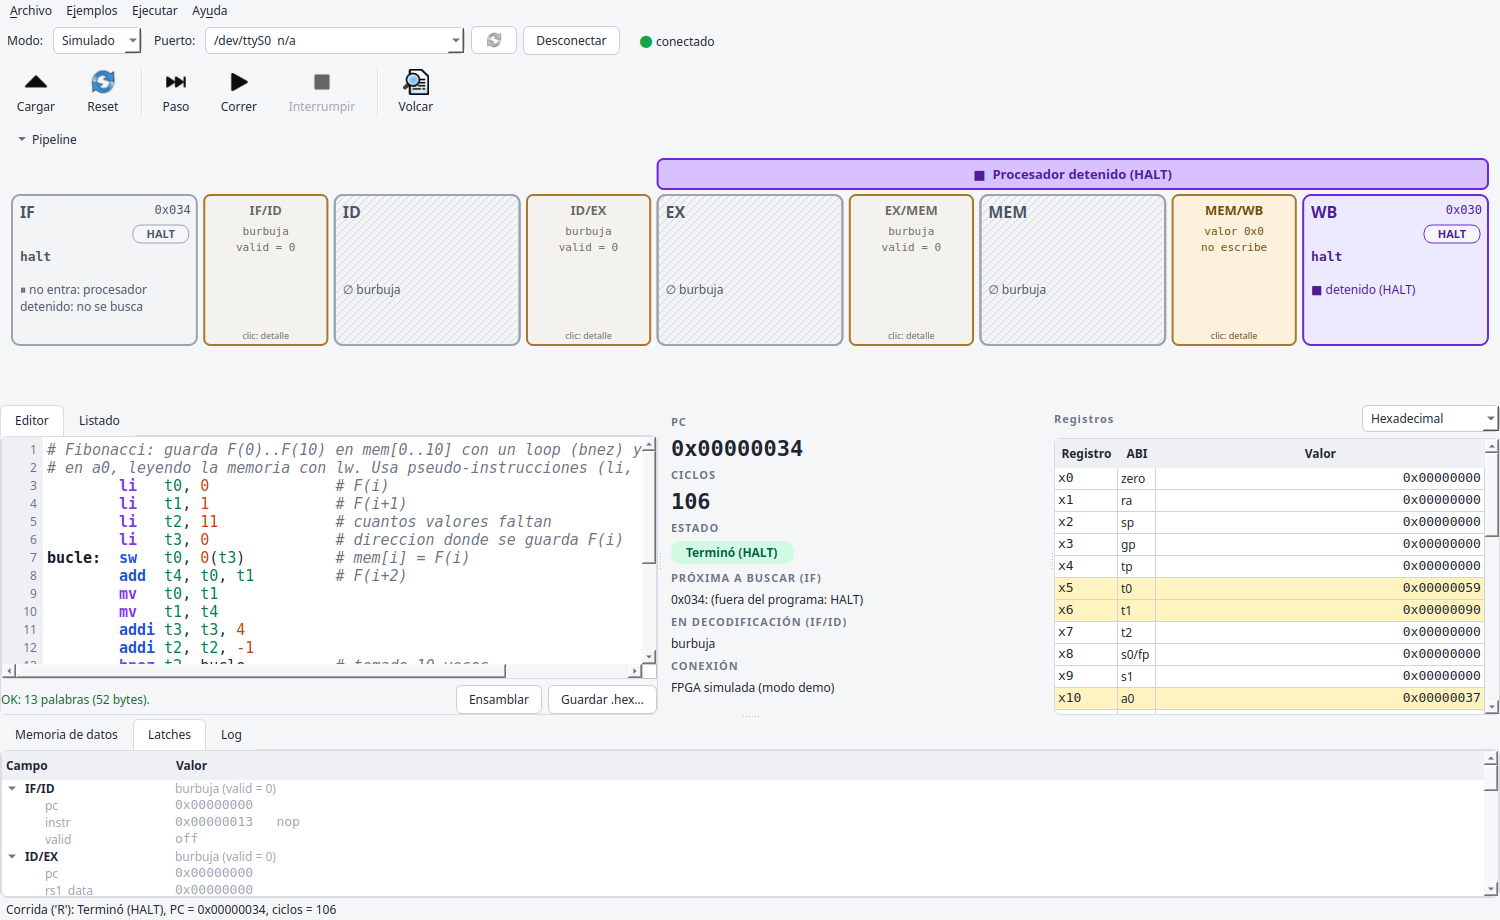
\includegraphics[width=\textwidth]{depurador_latches.png}
  \caption{Procesador detenido por HALT: pipeline vacío (burbujas en IF/ID,
  ID/EX y EX/MEM) y, abajo, el detalle de los registros de pipeline del
  volcado.}
  \label{fig:halt}
\end{figure}

El procesador también se detiene, con \texttt{o\_fault} = 1, ante una
instrucción no soportada, un fetch fuera de la memoria de programa o
desalineado, o un acceso inválido a la memoria de datos. Las instrucciones
anteriores terminan y la que falla, junto con las posteriores, no tiene
efectos. La Debug Unit informa el error en el byte de estado (0x05, distinto
del HALT normal 0x01).

\subsubsection{Clock enable y reset}

Todo el estado del procesador ---PC, registros de pipeline, banco de
registros, escrituras a la memoria de datos y el registro de parada--- se
habilita con
\(\texttt{step} = \texttt{i\_enable} \land \lnot\texttt{o\_halted}\). El clock
nunca se toca. Con \texttt{o\_halted} = 1 nada avanza y el estado queda estable
para el volcado. El reset es sincrónico y tiene prioridad sobre la habilitación.

\subsection{Debug Unit y comunicación (parte B)}

\begin{figure}[H]
  \centering
  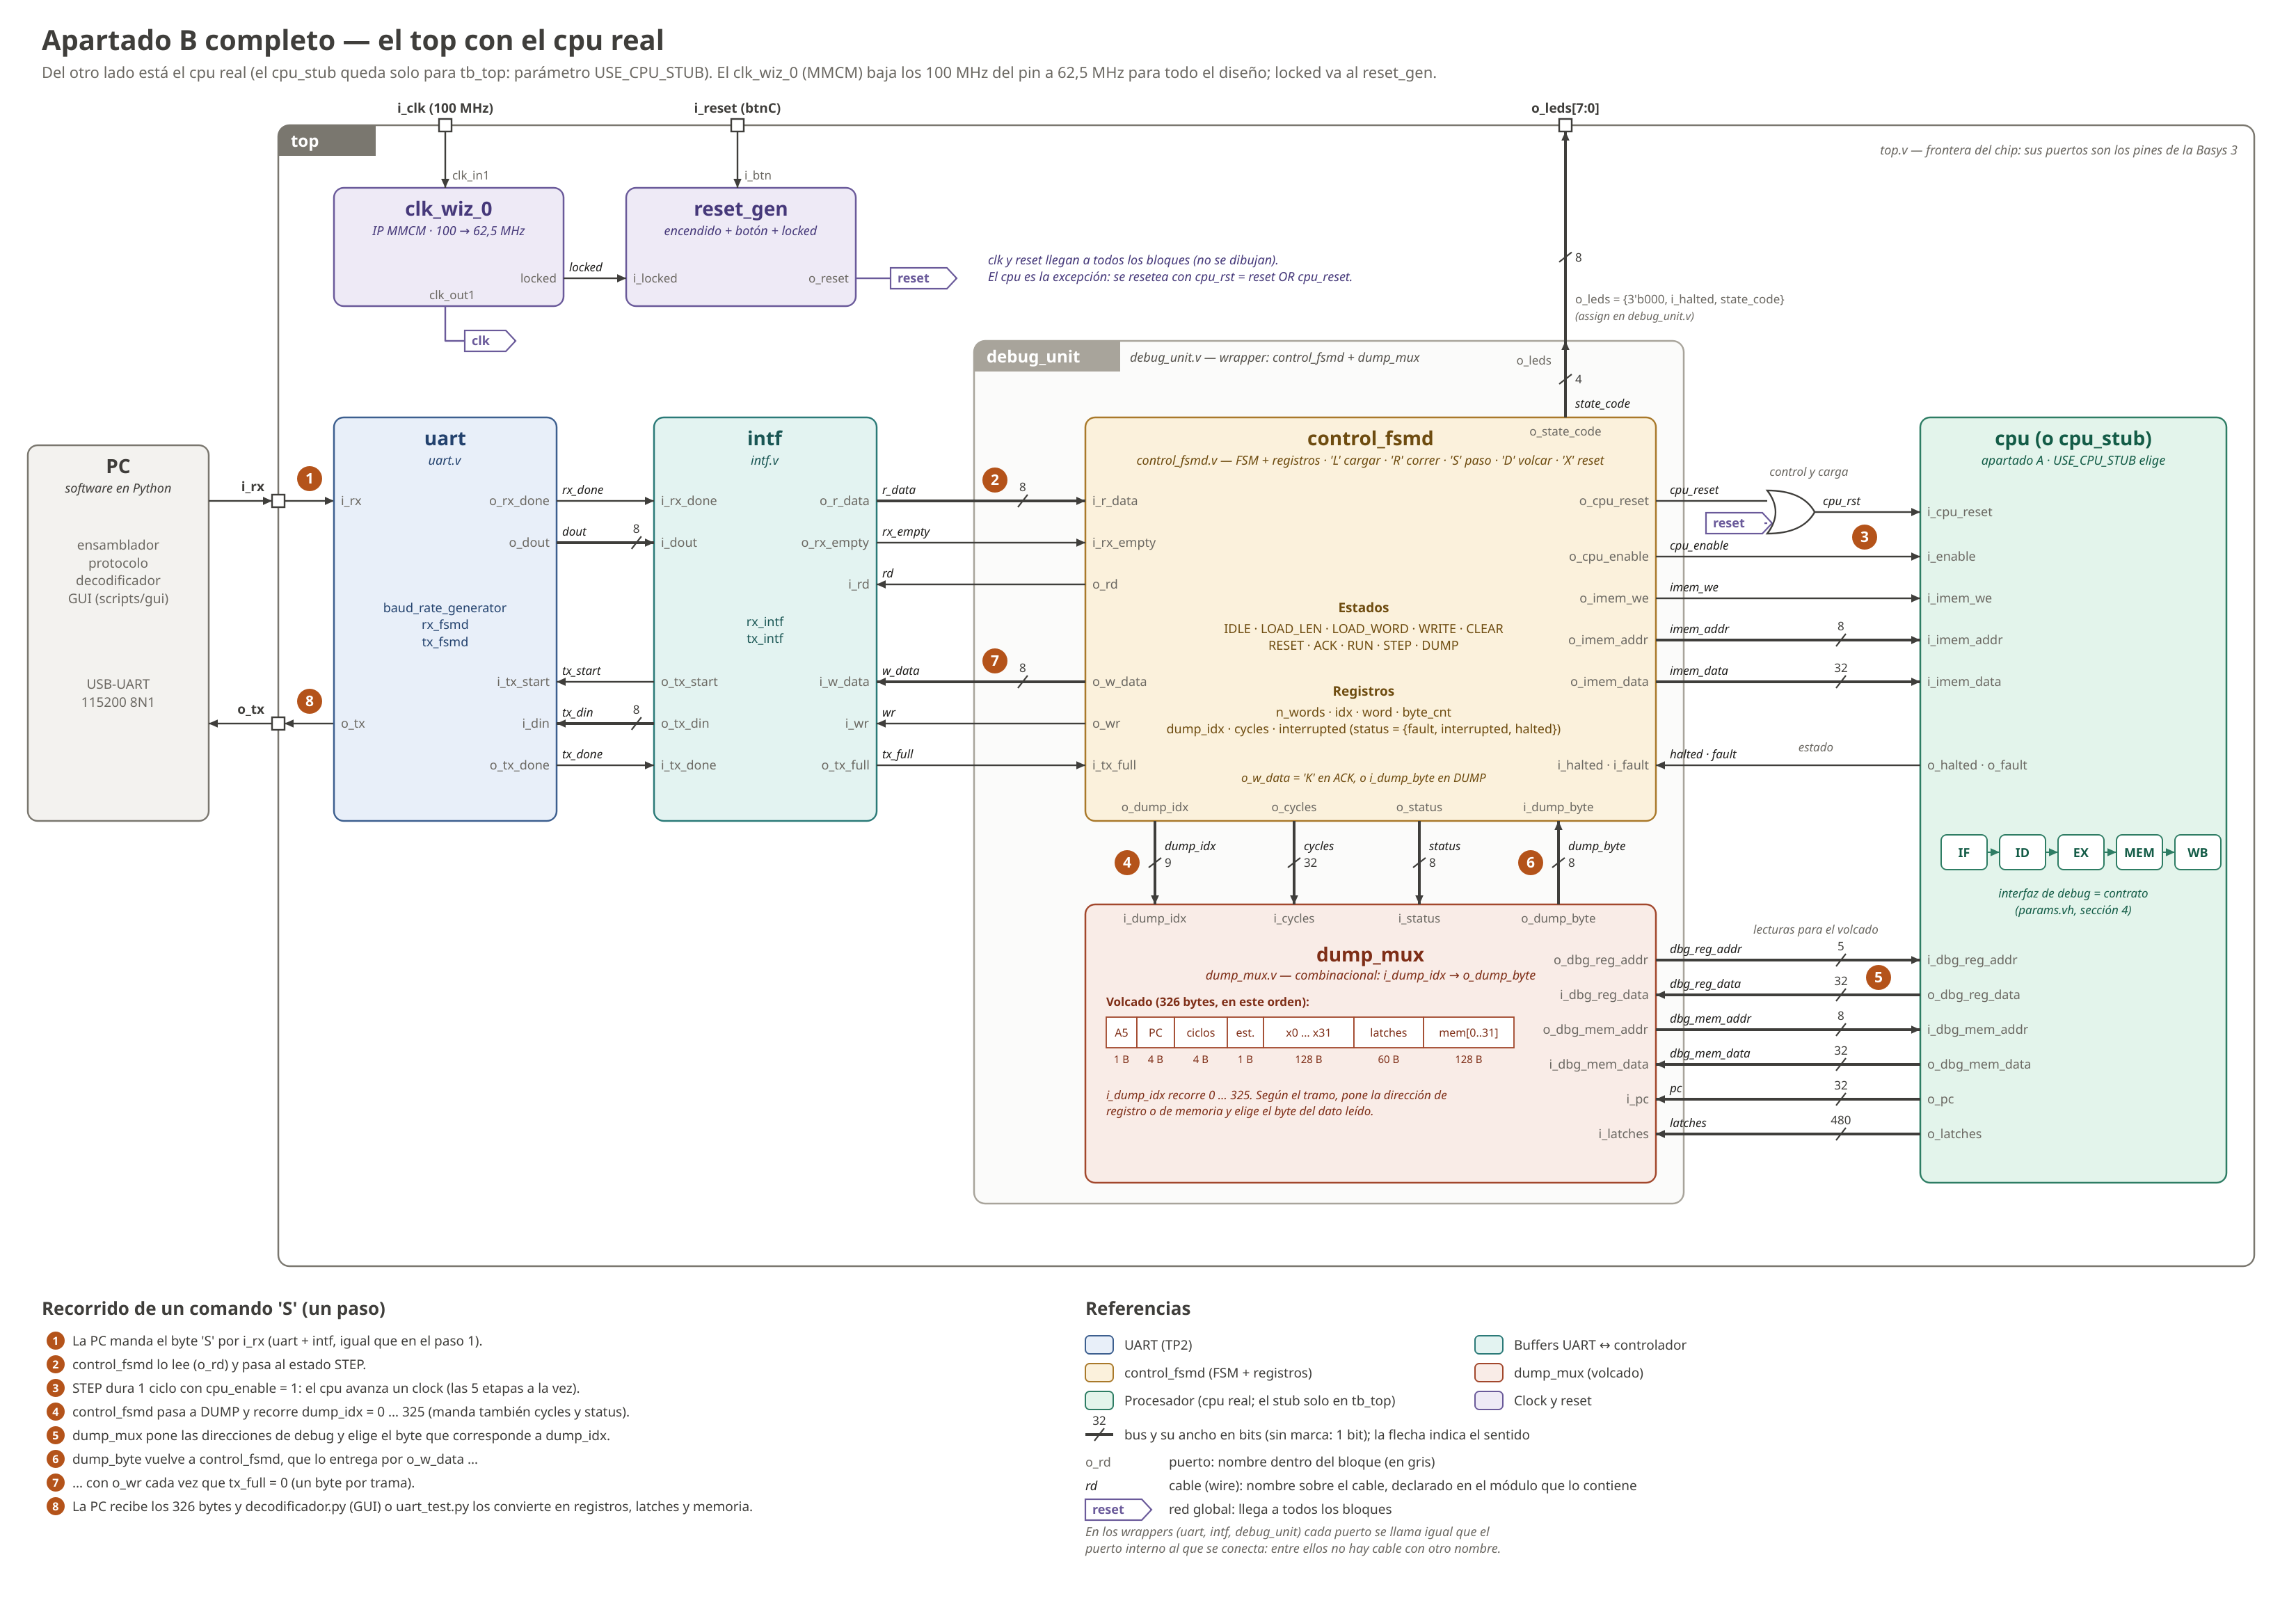
\includegraphics[width=\textwidth]{B_completo.png}
  \caption{Top de la parte B: UART, buffers de interfaz, Debug Unit
  (\texttt{control\_fsmd} y \texttt{dump\_mux}) y procesador, con el recorrido de
  un comando de paso.}
  \label{fig:parteB}
\end{figure}

\subsubsection{UART e interfaz}

La UART (\texttt{uart} = \texttt{baud\_rate\_generator} + \texttt{rx\_fsmd} +
\texttt{tx\_fsmd}) trabaja a 115\,200~baudios, 8N1, con sobremuestreo $\times 16$.
El generador produce un pulso de un ciclo 16~veces por bit, que las máquinas
de estados usan como \emph{habilitación} (no es un clock). El divisor se
redondea al entero más cercano; a 62,5~MHz es
$\mathrm{round}(62\,500\,000 / (115\,200 \cdot 16)) = \mathrm{round}(33{,}9) = 34$,
con un baud real de $62\,500\,000 / (34 \cdot 16) \approx 114\,890$ y un error de
$-0{,}27\%$, muy por debajo del límite tolerable ($\approx 2\%$). La línea \texttt{i\_rx} pasa por un sincronizador de dos
flip-flops. Entre la UART y la Debug Unit, el módulo \texttt{intf} tiene un
buffer de un byte en cada sentido, con un \emph{handshake}
\texttt{rd}/\texttt{rx\_empty} y \texttt{wr}/\texttt{tx\_full}. Alcanza con un
byte porque la FSM consume cada byte al ciclo siguiente y el próximo tarda
$\approx 87~\mu$s en llegar.

\subsubsection{Protocolo}

La comunicación es de tipo pedido $\rightarrow$ respuesta, con comandos de un
byte ASCII:

\begin{table}[H]
\centering
\small
\begin{tabular}{@{}lL{8cm}l@{}}
\toprule
Comando & Acción & Respuesta \\
\midrule
\cmd{L} + N + palabras & carga N palabras en la memoria de programa, completa el resto con HALT y resetea el procesador & \cmd{K} \\
\cmd{X} & reset del procesador (la UART no se resetea) & \cmd{K} \\
\cmd{D} & volcado, sin ejecutar & volcado \\
\cmd{S} & un ciclo de clock habilitado & volcado \\
\cmd{R} & corre hasta el HALT (o hasta \cmd{I}) & volcado \\
\cmd{I} & interrumpe un \cmd{R} en curso; fuera de él se ignora & (el del \cmd{R}) \\
\bottomrule
\end{tabular}
\caption{Protocolo entre la PC y la Debug Unit.}
\end{table}

El volcado tiene 326~bytes, todos los valores en little-endian:

\begin{table}[H]
\centering
\small
\begin{tabular}{@{}rrL{9cm}@{}}
\toprule
Offset & Bytes & Contenido \\
\midrule
0 & 1 & cabecera \texttt{0xA5} \\
1 & 4 & PC \\
5 & 4 & contador de ciclos habilitados \\
9 & 1 & estado: bit~0 detenido, bit~1 interrumpido, bit~2 error \\
10 & 128 & registros \texttt{x0}..\texttt{x31} \\
138 & 60 & registros de pipeline (480~bits) \\
198 & 128 & memoria de datos, palabras 0..31 \\
\bottomrule
\end{tabular}
\caption{Formato del volcado (326~bytes, $\approx 28$~ms a 115\,200~baudios).}
\end{table}

\subsubsection{Máquina de estados}

La Debug Unit se dividió en dos bloques de naturaleza distinta:
\texttt{control\_fsmd}, la máquina de estados con sus registros (el protocolo),
y \texttt{dump\_mux}, combinacional, que dado el índice de un byte del volcado
lo arma y pone las direcciones de lectura de debug. El volcado se genera ``al
vuelo'', sin un buffer de 326~bytes: como el procesador está congelado durante
la transmisión, todos los bytes corresponden al mismo instante.

\begin{figure}[H]
  \centering
  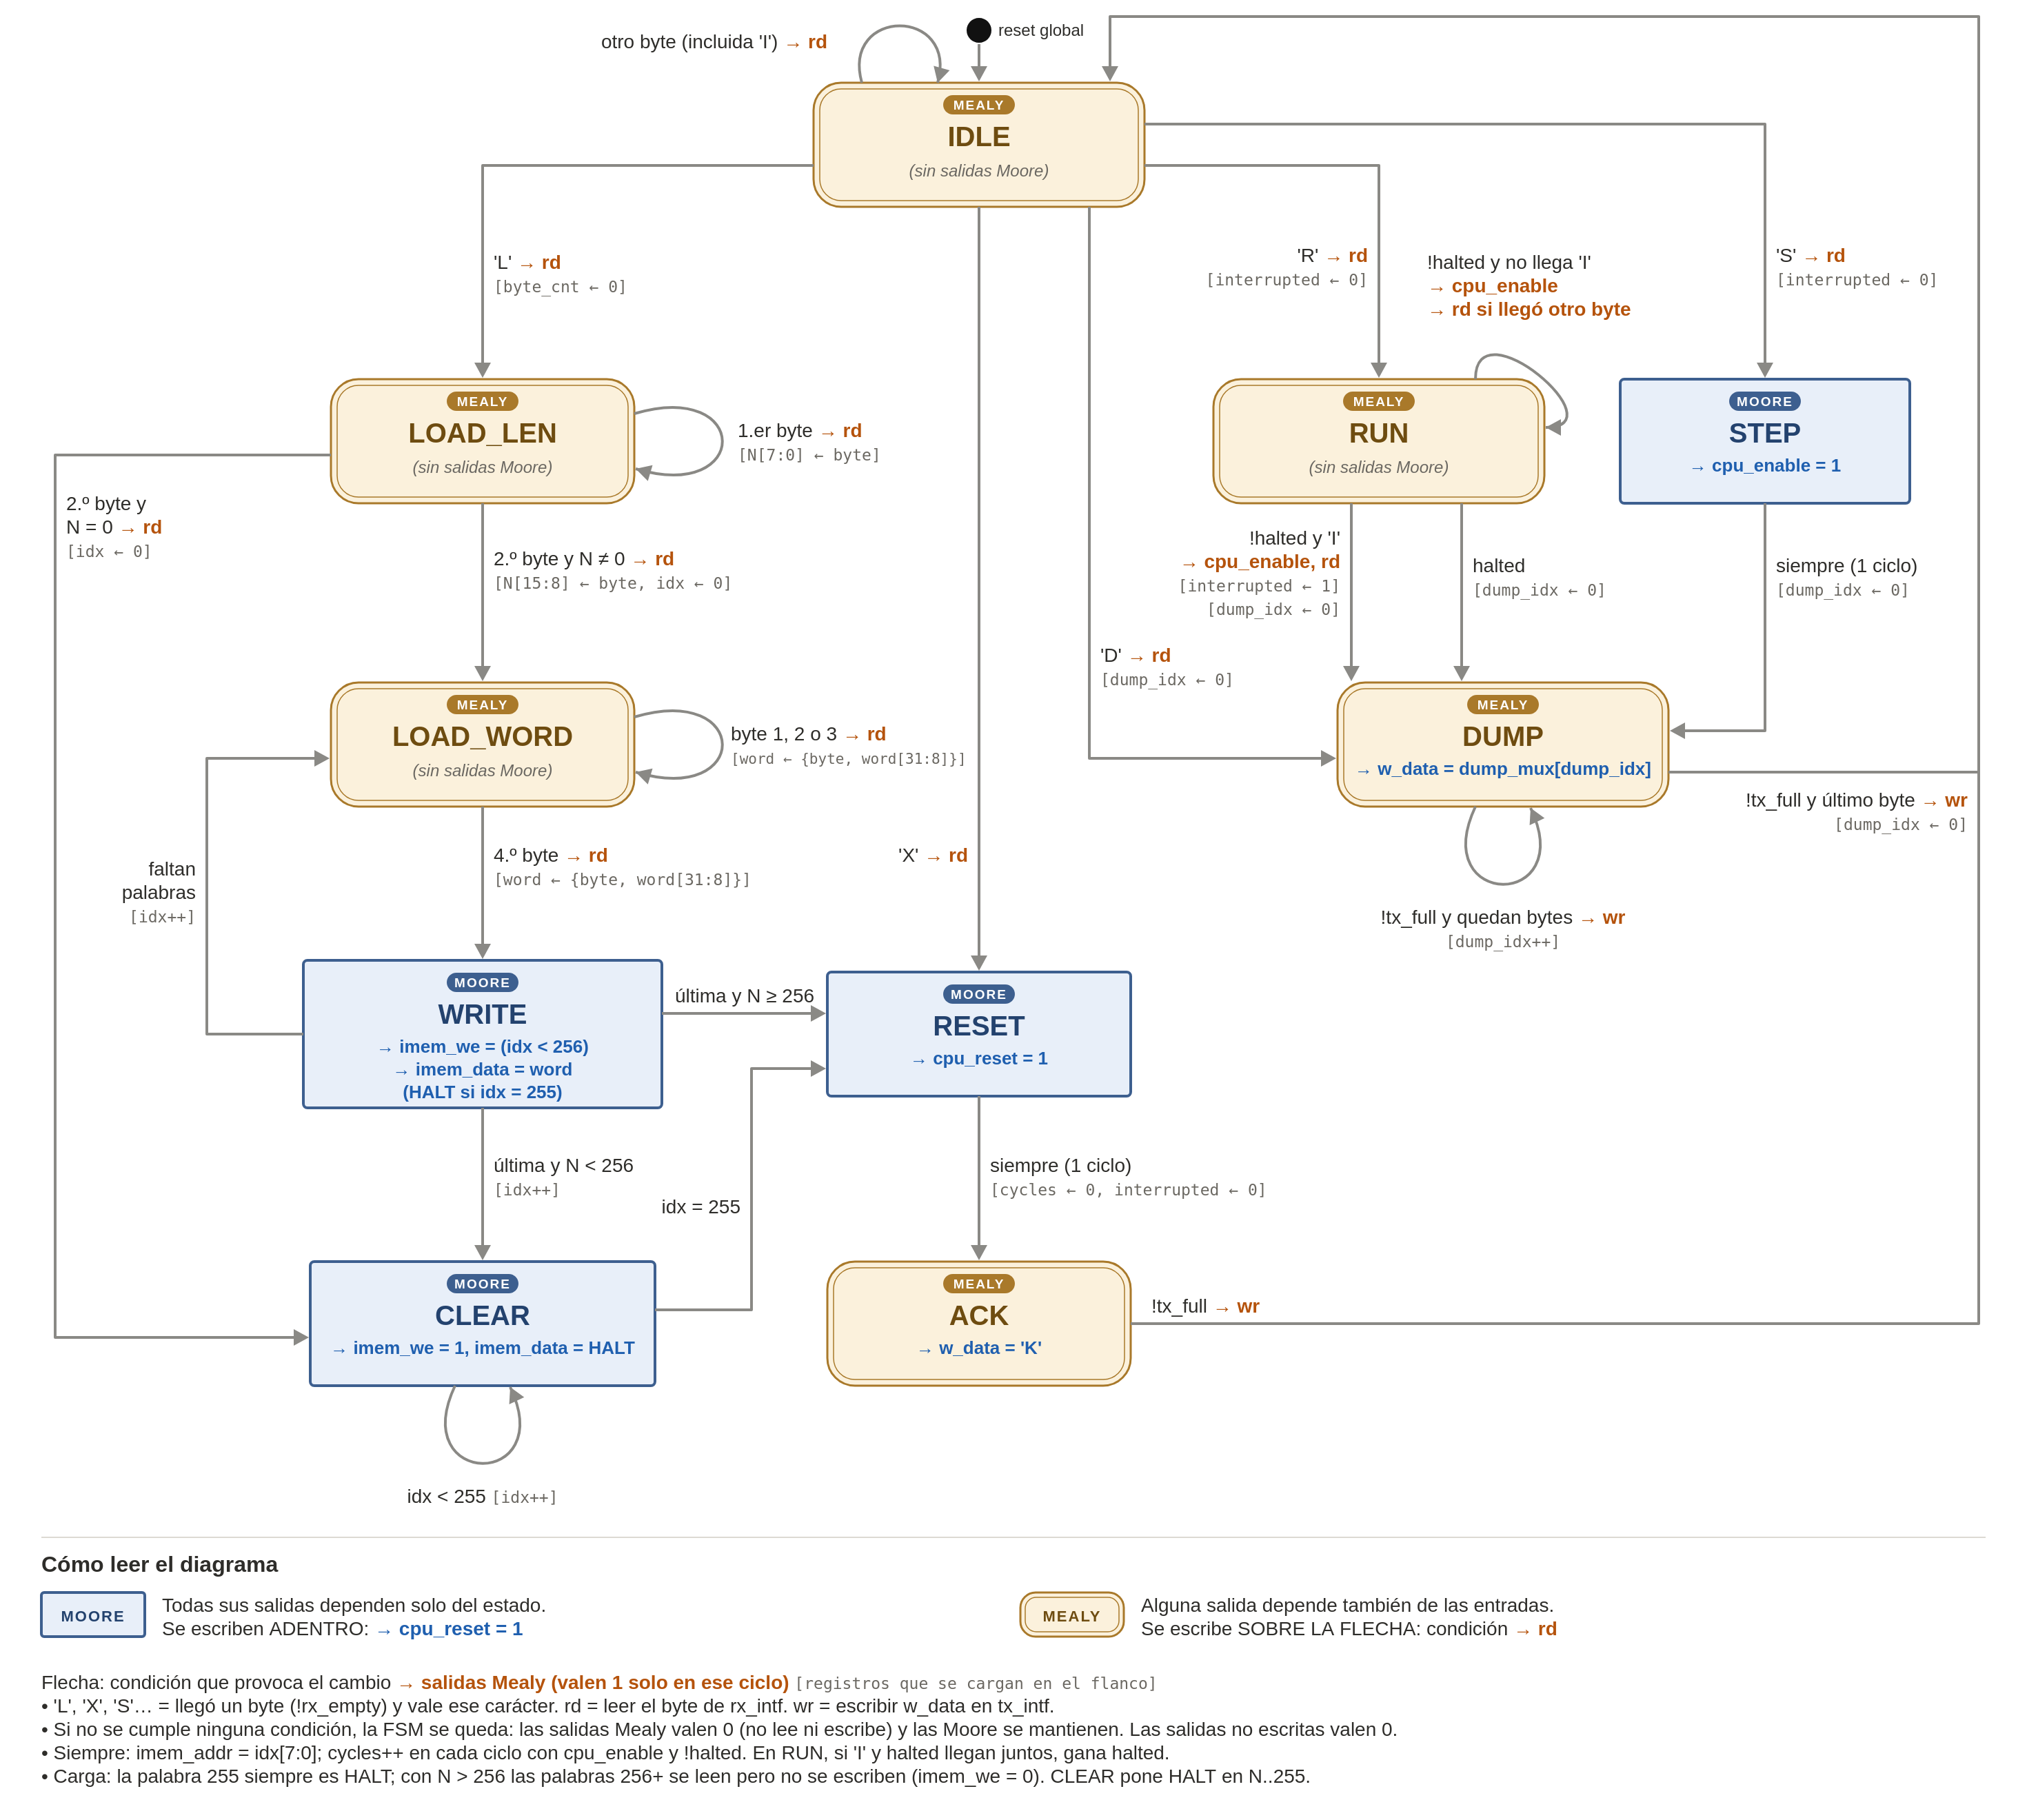
\includegraphics[width=\textwidth]{debug_unit_fsm_v2.png}
  \caption{Diagrama de estados de \texttt{control\_fsmd}.}
  \label{fig:fsm}
\end{figure}

La figura~\ref{fig:fsm} muestra los diez estados (codificación one-hot, con
recuperación a IDLE ante un estado inválido). Las salidas que controlan al
procesador son de tipo \textbf{Moore}: dependen solo del estado y duran
exactamente lo que dura el estado. Por eso el estado STEP, de un ciclo, da un
único flanco habilitado (el modo paso a paso). Las salidas del handshake son
\textbf{Mealy}, igual que el enable en RUN
(\(\texttt{cpu\_enable} = \lnot\texttt{halted}\)): en el mismo ciclo en que el
procesador se detiene, el enable baja y el contador de ciclos queda exacto. Si
\cmd{I} y el HALT llegan en el mismo ciclo, gana el HALT.

La carga (\cmd{L}) recibe la cantidad de palabras N en dos bytes y luego las
palabras, todo seguido. Cada palabra se arma con un registro de desplazamiento
(\texttt{word = \{byte, word[31:8]\}}, little-endian) y se escribe en un ciclo
(estado WRITE). El estado CLEAR escribe HALT en todas las palabras que el
programa no usa, y la palabra 255 siempre es HALT. Durante la carga ningún byte
se interpreta como comando, y con N > 256 las palabras sobrantes se consumen
sin escribirse, para no desincronizar el protocolo.

\subsubsection{Reset y reloj}

El módulo \texttt{reset\_gen} genera el reset global: durante 16~ciclos al
encender, mientras se aprieta el botón (sincronizado) y mientras el MMCM no
está enganchado (\texttt{locked} = 0). El procesador se resetea con
\(\texttt{cpu\_rst} = \texttt{reset} \lor \texttt{cpu\_reset}\): el comando \cmd{X}
reinicia solo el procesador y la comunicación sigue funcionando. El clock de
100~MHz del pin W5 entra únicamente al Clocking Wizard, que genera los 62,5~MHz
de todo el diseño (sección~\ref{sec:timing}). Un único clock evita cruces entre
dominios.

\subsection{Software de PC (parte C)}

\subsubsection{Ensamblador}

\texttt{scripts/ensamblador.py} traduce ensamblador a palabras de 32~bits en
dos pasadas: la primera calcula la dirección de cada etiqueta y la segunda
codifica cada instrucción campo por campo según su formato. Acepta las
instrucciones de la consigna, \texttt{halt}, etiquetas, comentarios y las
pseudo-instrucciones \texttt{nop}, \texttt{j}, \texttt{mv}, \texttt{li} (una o
dos palabras), \texttt{beqz}, \texttt{bnez}, \texttt{call} y \texttt{ret}. Las
instrucciones RISC-V que no están en la consigna dan un error explícito con el
número de línea. Se prefirió un ensamblador propio frente a la toolchain de GNU
o RARS porque el HALT no es estándar, porque se quería rechazar lo que el
procesador no implementa y porque se necesitaba generar directamente el formato
de carga. Se validó contra el ensamblador de GNU: el programa de cobertura de
la parte~A produce las mismas 39 palabras.

\subsubsection{Modelo de referencia}

\texttt{scripts/rv32i\_model.py} ejecuta el programa por su cuenta, sin usar el
RTL: decodifica cada instrucción y calcula los tiempos del pipeline con las
reglas de la sección anterior. Obtiene los registros, la memoria, el PC y el
estado después de \emph{cada} ciclo. Es la fuente de los valores esperados de
los testbenches, de modo que el hardware no se compara contra sí mismo.

\subsubsection{Depurador gráfico}

El depurador (\texttt{scripts/gui/}, PySide6) permite escribir y ensamblar
programas, cargarlos, ejecutarlos en ambos modos y ver el estado completo del
procesador sin usar la consola (figura~\ref{fig:gui}). La comunicación serie
corre en un hilo aparte, así la interfaz nunca se bloquea, y los errores se
muestran en la ventana y en un registro de eventos. Un \emph{modo simulado}
reemplaza la placa por una FPGA simulada que habla el mismo protocolo, byte a
byte, sobre un simulador del procesador ciclo a ciclo
(\texttt{pipeline\_sim.py}) que reproduce los 480~bits de los registros de
pipeline igual que el RTL. La herramienta de consola \texttt{uart\_test.py}
ofrece la misma funcionalidad por terminal.

\begin{figure}[H]
  \centering
  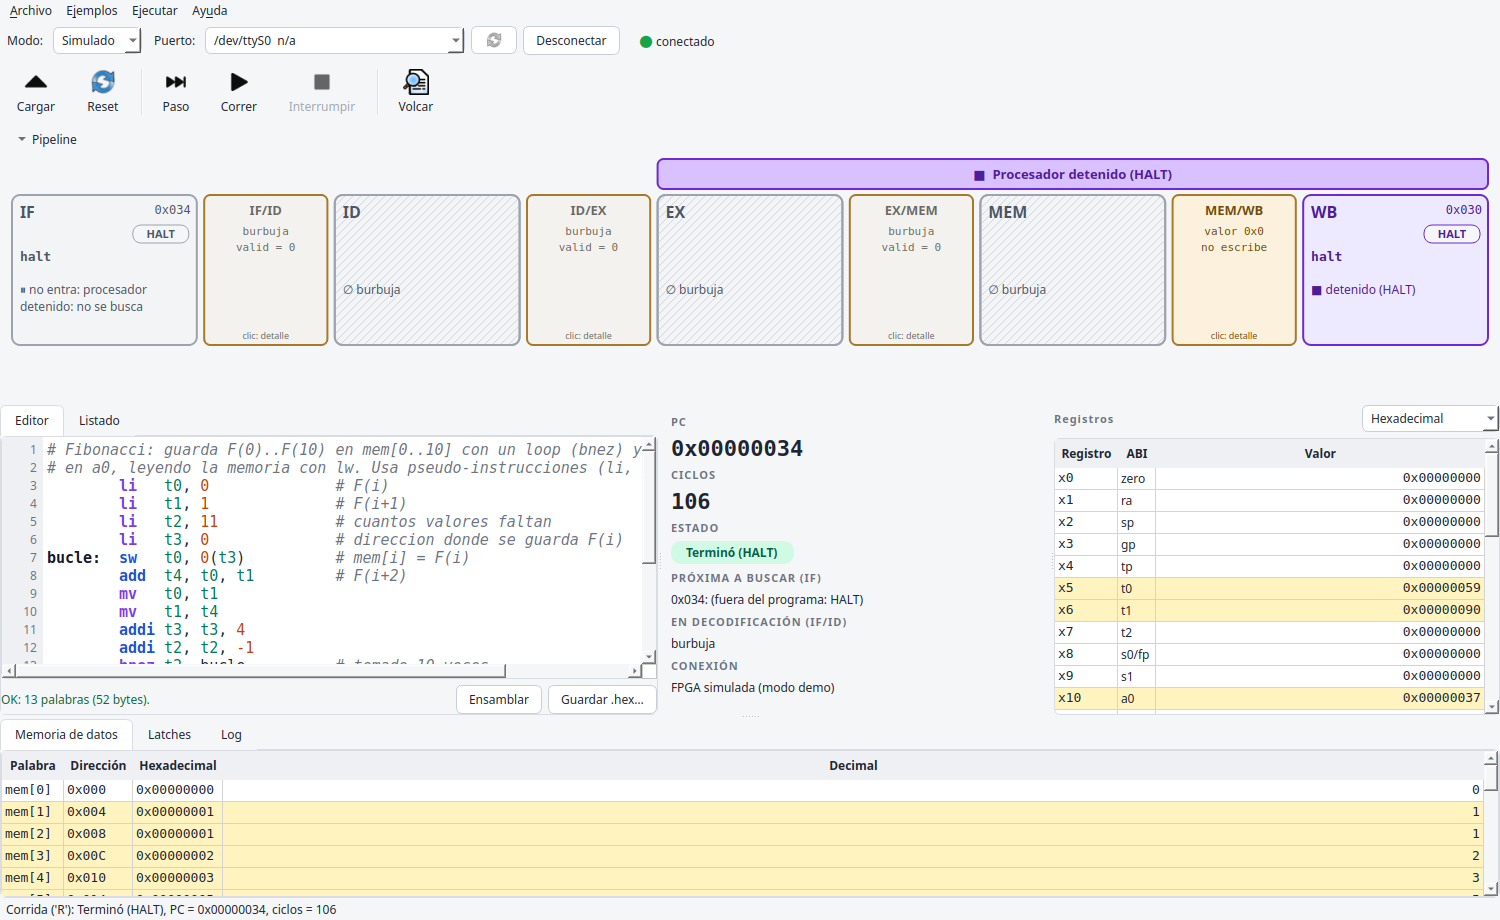
\includegraphics[width=\textwidth]{depurador_corrida.png}
  \caption{Depurador gráfico: vista del pipeline (arriba), listado del programa,
  PC, ciclos y estado, registros y memoria de datos, al terminar un programa.}
  \label{fig:gui}
\end{figure}

La \textbf{vista del pipeline} muestra qué instrucción hay en cada etapa y qué
está ocurriendo: flechas de forwarding, avisos de stall y de flush,
instrucciones que se van a descartar y burbujas con su origen. Como los
registros de pipeline guardan el PC solo en IF/ID e ID/EX, la instrucción en MEM
y en WB se deduce. Con dos volcados consecutivos la deducción es exacta, porque
EX/MEM y MEM/WB avanzan en todo flanco habilitado. En otro caso se simula desde
el reset y se usa el resultado solo si los 480~bits coinciden con el volcado; si
no hay certeza, la etapa se muestra como ``?''. La figura~\ref{fig:stall}
muestra un load-use: el aviso de stall y, en el ciclo siguiente, la burbuja.

\begin{figure}[H]
  \centering
  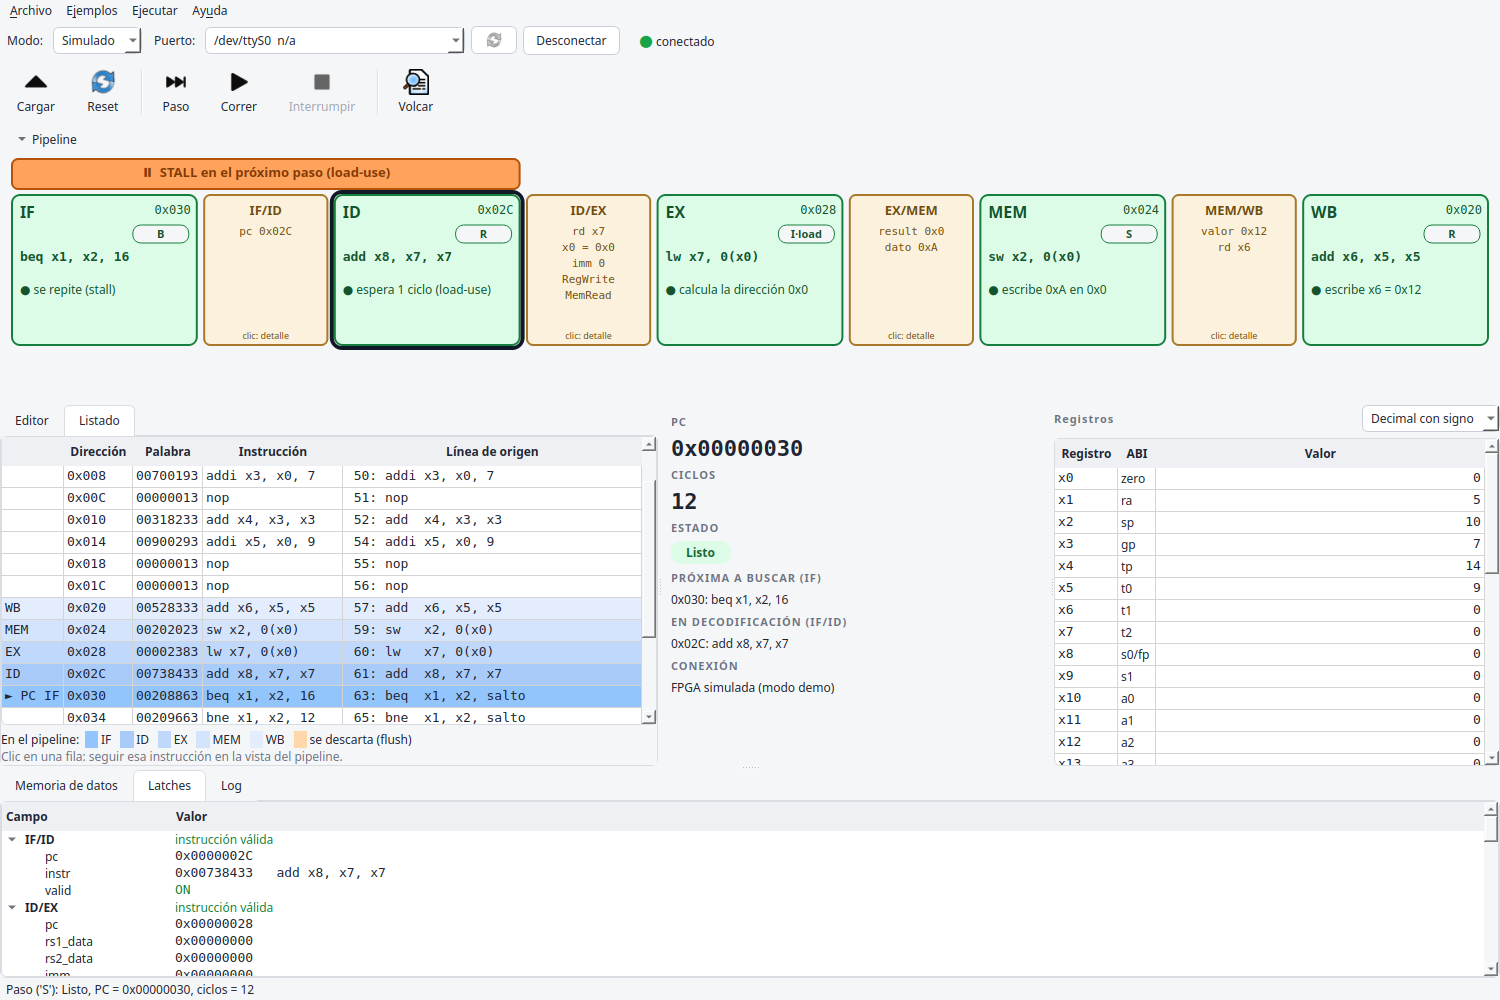
\includegraphics[width=0.49\textwidth]{defensa_paso12_stall_aviso.png}\hfill
  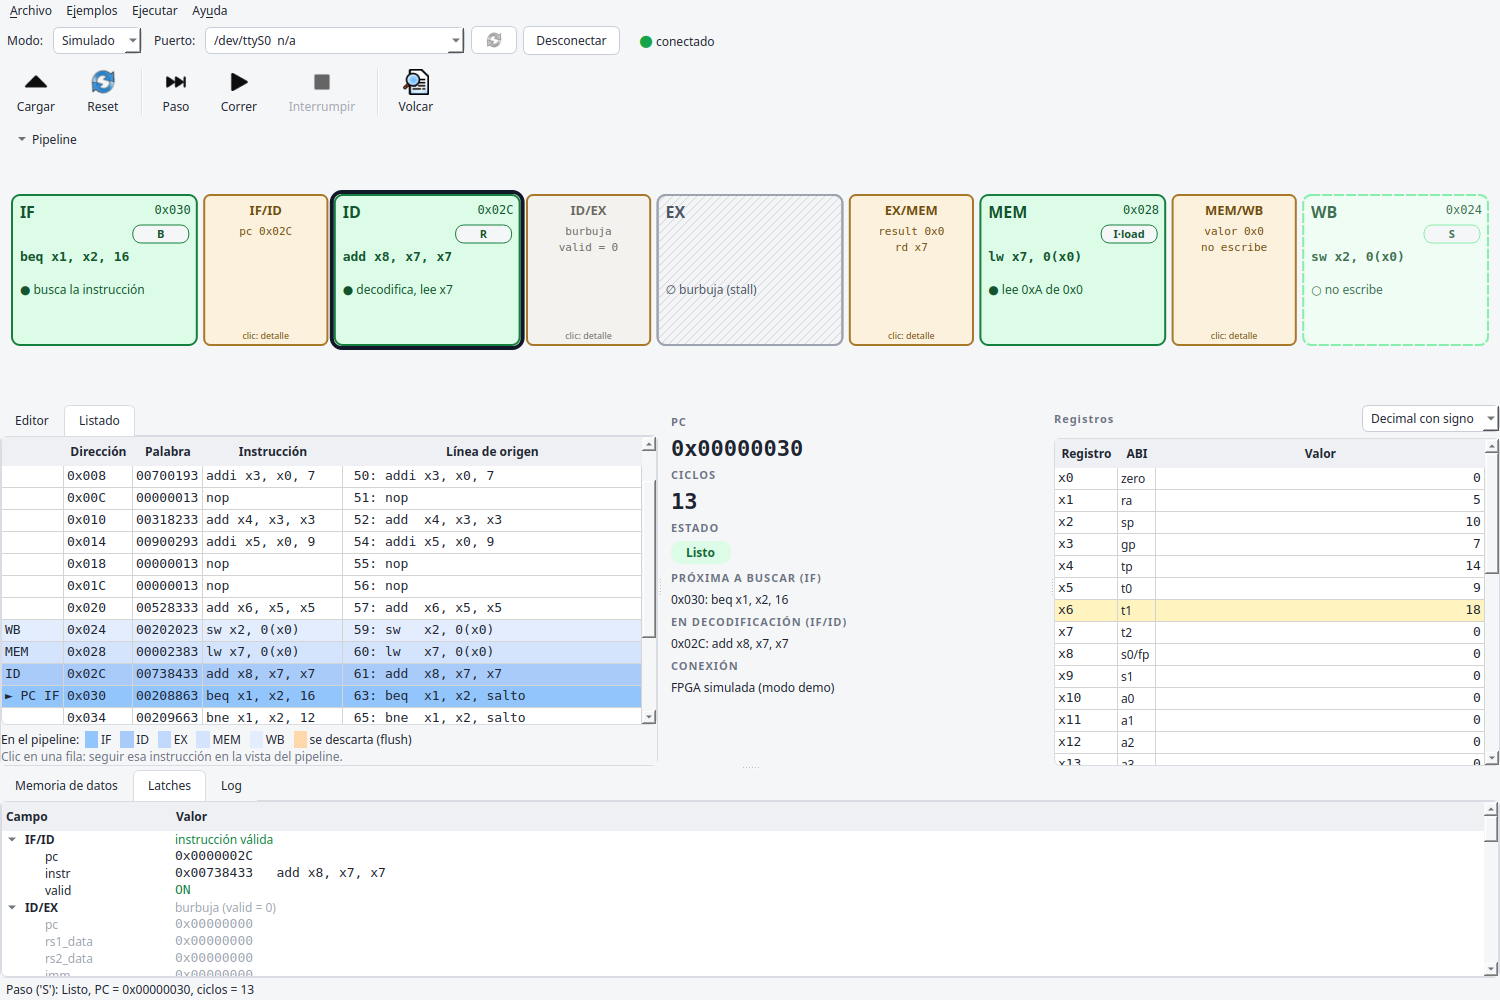
\includegraphics[width=0.49\textwidth]{defensa_paso13_stall_burbuja.png}
  \caption{Load-use en la vista del pipeline: a la izquierda, \texttt{lw x7} en
  EX y \texttt{add x8, x7, x7} en ID, con el aviso de stall; a la derecha, la
  burbuja en EX con IF e ID congelados.}
  \label{fig:stall}
\end{figure}

% ============================================================
\section{Verificación}
% ============================================================

\subsection{Estrategia}

Todos los testbenches son \textbf{autoverificados}: comparan solos contra lo
esperado e imprimen PASS o FAIL. Los valores esperados no salen del DUT sino de
tres fuentes independientes que se cruzan entre sí: cuentas hechas a mano
(anotadas en cada programa de ejemplo), el modelo de referencia y el RTL. Los
testbenches que pasan por la UART simulan a 1~Mbaud mediante un parámetro (el
diseño sigue en 115\,200) para reducir el tiempo de simulación. Todo el RTL
compila con \texttt{iverilog -Wall -g2005} sin warnings, y Verilator no reporta
latches inferidos, lazos combinacionales ni señales con más de un driver.

\begin{table}[H]
\centering
\small
\begin{tabular}{@{}L{4cm}L{11.4cm}@{}}
\toprule
Testbench & Qué verifica \\
\midrule
Módulos de la parte A & banco de registros, registros de pipeline, forwarding, hazard, memoria de datos e IF/ID por separado \\
\texttt{tb\_cpu} & el procesador completo con un programa largo, también pausando en cada ciclo; casos de error \\
\texttt{tb\_cpu\_isa} & el procesador contra el contrato (latencia del HALT, stall exacto, flush, enable en cero durante 50 ciclos, reset) y contra el modelo, \textbf{ciclo a ciclo}, en 11 programas \\
\texttt{tb\_top\_cpu} & el sistema completo por UART (\cmd{L}, \cmd{R}, \cmd{D}, \cmd{S}, \cmd{I}) contra el modelo \\
\texttt{tb\_top}, \texttt{tb\_dump\_mux}, \texttt{tb\_cpu\_stub} & el protocolo de la Debug Unit y el volcado byte a byte \\
\bottomrule
\end{tabular}
\caption{Testbenches del hardware (\texttt{scripts/run\_all\_tests.sh} los corre todos).}
\end{table}

El software tiene 1\,019 tests automáticos (pytest). Entre ellos, un testbench
propio captura los bytes que manda la FPGA simulada en Icarus y verifica que el
decodificador los interpreta campo por campo, y otro compara en cada ciclo los
480~bits de los registros de pipeline del RTL con los del simulador de la GUI.

\subsection{Programas de prueba}

\begin{table}[H]
\centering
\small
\begin{tabular}{@{}lL{6.6cm}rr@{}}
\toprule
Programa & Qué ejercita & Ciclos & Estado \\
\midrule
\texttt{ejemplo\_3} & forwarding simple & 6 & 0x01 \\
\texttt{nops\_5} & latencia del HALT & 9 & 0x01 \\
\texttt{sumas\_encadenadas} & forwarding EX/MEM, MEM/WB, bypass, \texttt{x0} & 18 & 0x01 \\
\texttt{alu} & todas las operaciones con casos borde & 36 & 0x01 \\
\texttt{memoria} & stores y loads de byte y media palabra, load-use & 34 & 0x01 \\
\texttt{saltos} & \texttt{beq}/\texttt{bne} tomados y no, \texttt{jal}/\texttt{jalr} & 28 & 0x01 \\
\texttt{loop\_bne} & loop de 10 vueltas, load-use antes de un salto & 63 & 0x01 \\
\texttt{error\_ilegal} & instrucción no soportada & 5 & 0x05 \\
\texttt{error\_lw} & load fuera de la memoria de datos & 6 & 0x05 \\
\texttt{NOPx256} & 256 NOP sin HALT: la palabra 255 se fuerza a HALT & 259 & 0x01 \\
\texttt{loop\_infinito} & programa sin fin, cortado con \cmd{I} & --- & 0x02 \\
\bottomrule
\end{tabular}
\caption{Programas de la integración: resultados idénticos en el modelo y en el RTL.}
\end{table}

Como ejemplo de un programa real, \texttt{demo\_wow\_fibonacci} llena las 32
palabras de la memoria de datos con la serie de Fibonacci
(\texttt{mem[31]} = 1\,346\,269): ejecuta 196 instrucciones con 31 saltos
tomados en $196 + 4 + 2 \cdot 31 = 262$ ciclos (CPI = 1,34), y el hardware
coincide con el modelo en cada ciclo (figura~\ref{fig:fib}). En
\texttt{demo\_pipeline}, cada fenómeno aparece en un paso conocido y verificado:
forwarding EX/MEM en el paso~3, MEM/WB en el~6, bypass en el~9, stall en el~12
(burbuja en el~13), flush en el~16 y HALT en WB en el~22, con un total de
$15 + 4 + 1 + 2 = 22$ ciclos.

\begin{figure}[H]
  \centering
  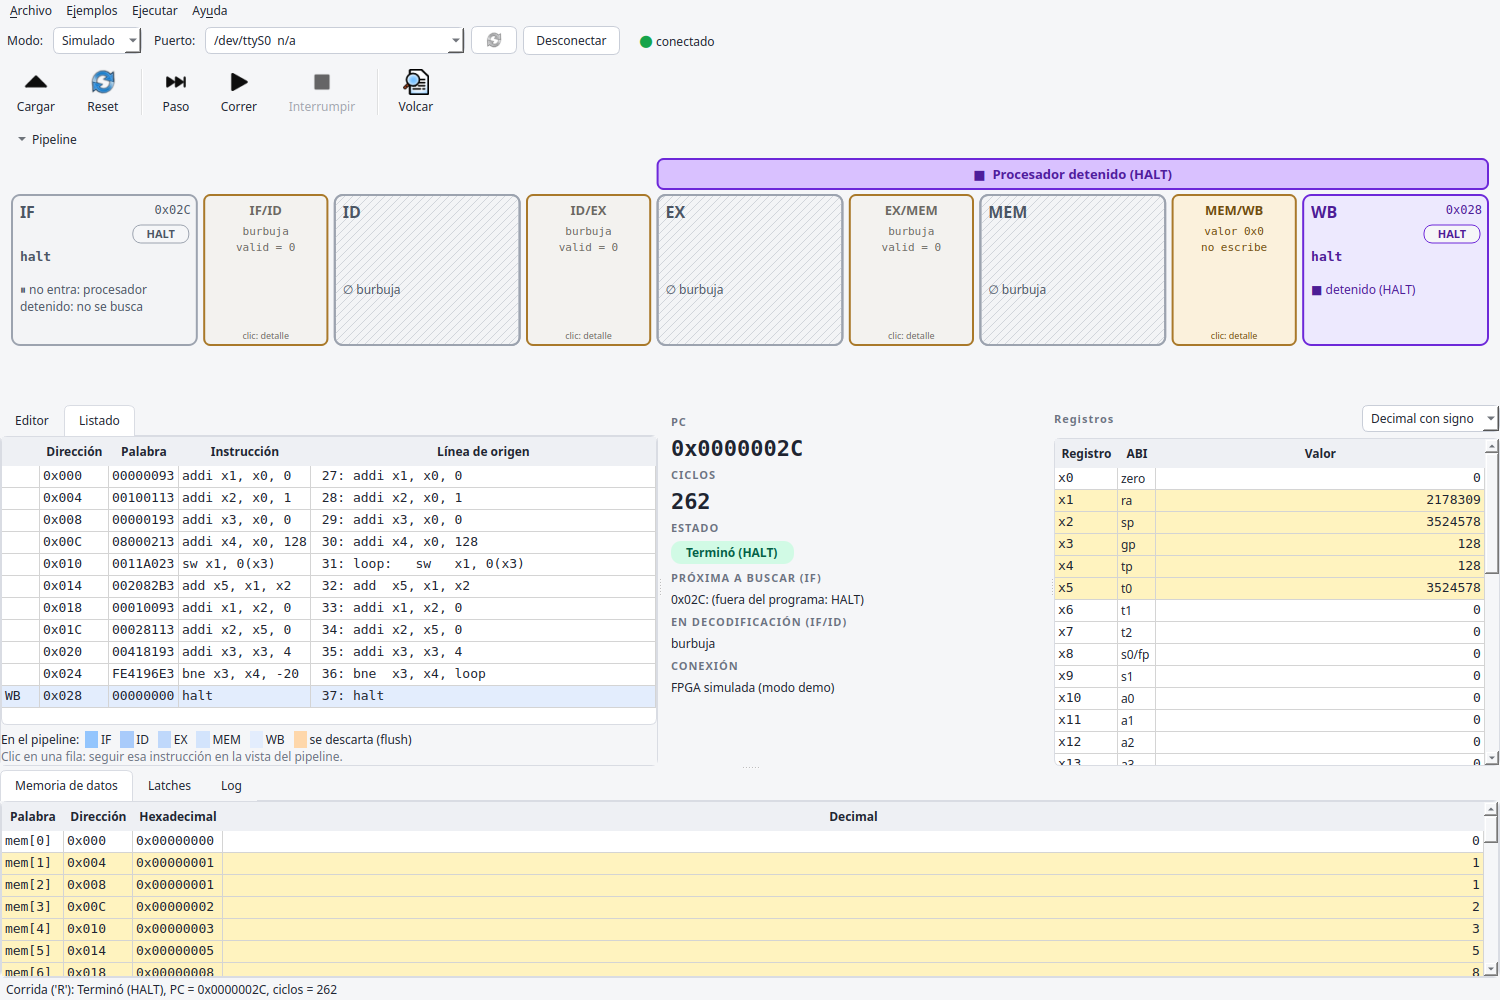
\includegraphics[width=\textwidth]{defensa_wow_fibonacci.png}
  \caption{Fibonacci en memoria al terminar: 262 ciclos, memoria de datos
  llena y procesador detenido con el pipeline vacío.}
  \label{fig:fib}
\end{figure}

\subsection{Pruebas de mutación}

Para comprobar que los tests detectan errores, se introdujeron fallas a
propósito, de a una por vez, sobre una copia del diseño
(\texttt{scripts/mutaciones.py}). \textbf{Las 12 fueron detectadas.}

\begin{table}[H]
\centering
\small
\begin{tabular}{@{}rL{7.2cm}ccc@{}}
\toprule
\# & Mutación & \texttt{tb\_cpu\_isa} & \texttt{tb\_cpu} & \texttt{tb\_top\_cpu} \\
\midrule
1 & sin forwarding EX/MEM & detecta & detecta & detecta \\
2 & sin forwarding MEM/WB & detecta & detecta & detecta \\
3 & sin stall load-use & detecta & detecta & detecta \\
4 & sin flush de IF/ID & detecta & detecta & detecta \\
5 & sin flush de ID/EX & detecta & detecta & detecta \\
6 & enable ignorado en EX/MEM & detecta & detecta & --- \\
7 & HALT un ciclo tarde & detecta & detecta & detecta \\
8 & \texttt{lb} sin extensión de signo & detecta & detecta & detecta \\
9 & \texttt{sra} igual a \texttt{srl} & detecta & detecta & detecta \\
10 & sin bypass WB $\rightarrow$ ID & detecta & detecta & detecta \\
11 & el reset borra la memoria de datos & detecta & detecta & detecta \\
12 & el estado no informa el error & --- & --- & detecta \\
\bottomrule
\end{tabular}
\caption{Pruebas de mutación. La 6 no se ve por UART porque en un \cmd{R}
el enable está siempre en 1; la 12 está en la Debug Unit, que solo prueba
\texttt{tb\_top\_cpu}.}
\end{table}

\subsection{Problemas encontrados}

La verificación contra el contrato encontró diferencias en la integración, que
se corrigieron: el procesador subía \texttt{o\_halted} un ciclo tarde (10 en lugar
de 9 ciclos), el puerto de debug no forzaba \texttt{x0} a cero, y el contrato
declaraba una memoria de datos de 256~palabras mientras el procesador tenía 32.
Además se agregaron la señal \texttt{o\_fault} y el formato de 480~bits, y una
prueba de mutación que inicialmente no se detectaba llevó a agregar un control
que faltaba en \texttt{tb\_top\_cpu}. Por último, el programa \texttt{NOPx256},
que ocupa las 256 palabras sin ningún HALT, mostró que el simulador de la GUI no
aplicaba la regla de la Debug Unit de forzar HALT en la palabra 255: ejecutaba
los 256 NOP, buscaba en 0x400 y terminaba con error en 260 ciclos, mientras que
el RTL y el modelo terminan con HALT normal en 259. Se agregó esa regla al
simulador, con un test propio.

% ============================================================
\section{Implementación en la placa}
% ============================================================

\subsection{Conexión física}

La Basys~3 se conecta a la PC con un único cable USB, que alimenta la placa,
permite programarla (JTAG) y lleva la UART a través del puente FTDI. El puente
aparece en Linux como dos puertos serie (el de la UART es la segunda interfaz).
No se necesita ningún cableado adicional.

\subsection{Asignación de pines}

\begin{table}[H]
\centering
\small
\begin{tabular}{@{}lL{4.2cm}L{6.6cm}@{}}
\toprule
Puerto & Pin & Uso \\
\midrule
\texttt{i\_clk} & W5 & oscilador de 100~MHz (entrada del Clocking Wizard) \\
\texttt{i\_reset} & U18 & botón central (btnC): reset global \\
\texttt{i\_rx} & B18 & UART, de la PC a la FPGA \\
\texttt{o\_tx} & A18 & UART, de la FPGA a la PC \\
\texttt{o\_leds[0..7]} & U16, E19, U19, V19, W18, U15, U14, V14 & código de estado de la FSM (LD0--LD3) y \texttt{halted} (LD4) \\
\bottomrule
\end{tabular}
\caption{Asignación de pines (\texttt{constrains/top.xdc}).}
\end{table}

\subsection{Timing y frecuencia de trabajo}
\label{sec:timing}

\subsubsection{Primer intento: 100~MHz}
\label{sec:timing100}

El primer intento fue usar directamente el oscilador de 100~MHz de la placa,
sin Clocking Wizard: el clock entraba por el pin W5 y pasaba por un buffer de
entrada (IBUF) y un buffer global (BUFG) a todos los flip-flops, con una
restricción de período de 10~ns (\texttt{sys\_clk\_pin}). La implementación
\textbf{no cumple timing}: al abrir el diseño implementado Vivado emite la
advertencia crítica \texttt{[Timing 38-282]} (figura~\ref{fig:warn100}) y el
resumen de timing (figura~\ref{fig:wns100}) muestra 375 de los 6\,668
endpoints con slack de setup negativo.

\begin{figure}[H]
  \centering
  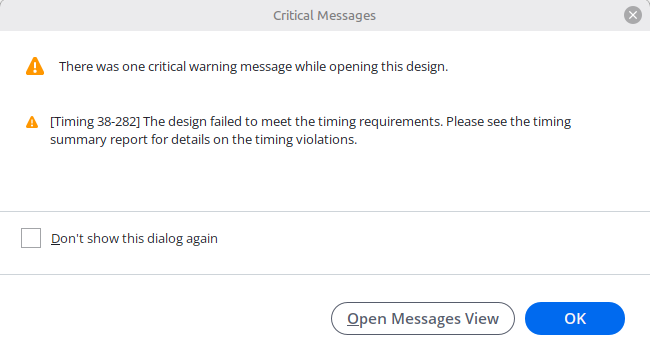
\includegraphics[width=0.6\textwidth]{timing.png}
  \caption{Advertencia crítica de Vivado a 100~MHz: el diseño no cumple los
  requisitos de timing.}
  \label{fig:warn100}
\end{figure}

\begin{figure}[H]
  \centering
  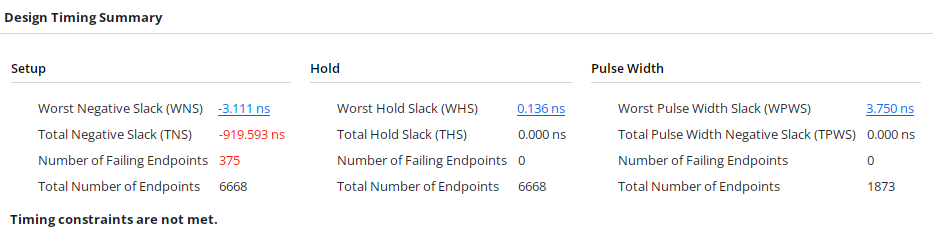
\includegraphics[width=\textwidth]{wns.png}
  \caption{Resumen de timing a 100~MHz: setup no cumple (WNS negativo); hold y
  ancho de pulso sí cumplen.}
  \label{fig:wns100}
\end{figure}

\begin{table}[H]
\centering
\small
\begin{tabular}{@{}ll@{}}
\toprule
Medida & Valor a 100~MHz \\
\midrule
WNS & $-3{,}111$~ns \\
TNS & $-919{,}593$~ns (375 de 6\,668 endpoints fallando) \\
WHS / THS & $+0{,}136$~ns / 0~ns (hold cumple) \\
WPWS & $+3{,}750$~ns (ancho de pulso cumple) \\
Camino crítico & \texttt{u\_id\_ex/o\_rs1\_reg[2]} $\rightarrow$ \texttt{u\_pc/o\_pc\_reg[30]} \\
Niveles de lógica & 21 (8 CARRY4, 2 LUT4, 5 LUT5, 6 LUT6, 1 MUXF7) \\
Retardo del camino & 13,021~ns: 3,899~ns de lógica (30\%) y 9,122~ns de ruteo (70\%) \\
Skew del camino & $-0{,}117$~ns \\
\bottomrule
\end{tabular}
\caption{Resultado de timing a 100~MHz, sin Clocking Wizard.}
\end{table}

La figura~\ref{fig:paths100} lista los diez peores caminos. Todos parten del
mismo flip-flop, el bit~2 del operando \texttt{rs1} guardado en ID/EX, y
terminan en distintos bits del PC: es un único camino lógico que se abre hacia
los 32~bits del próximo PC. Todos tienen el mismo retardo de ruteo (9,122~ns) y
entre 19 y 21 niveles de lógica.

\begin{figure}[H]
  \centering
  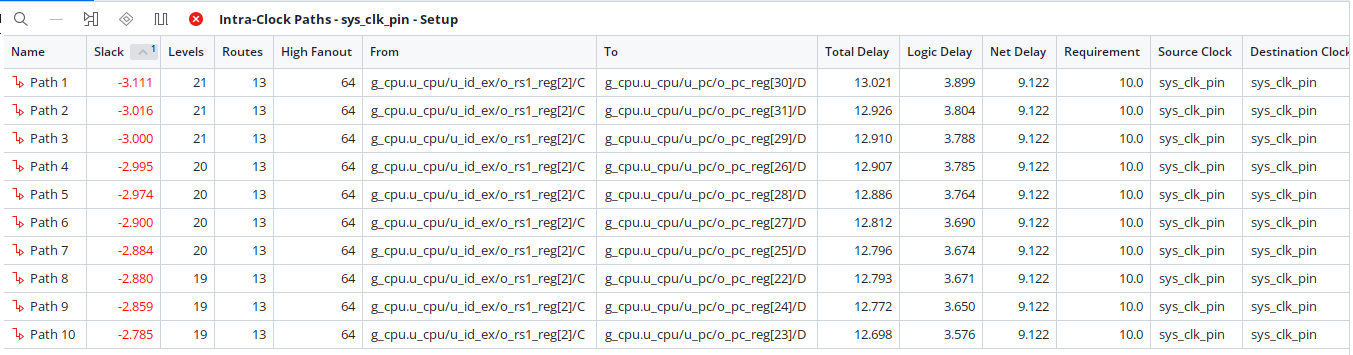
\includegraphics[width=\textwidth]{timing-path.png}
  \caption{Los diez caminos con peor slack a 100~MHz: todos van de
  \texttt{u\_id\_ex/o\_rs1\_reg[2]} a un bit de \texttt{u\_pc/o\_pc\_reg}.}
  \label{fig:paths100}
\end{figure}

\begin{figure}[H]
  \centering
  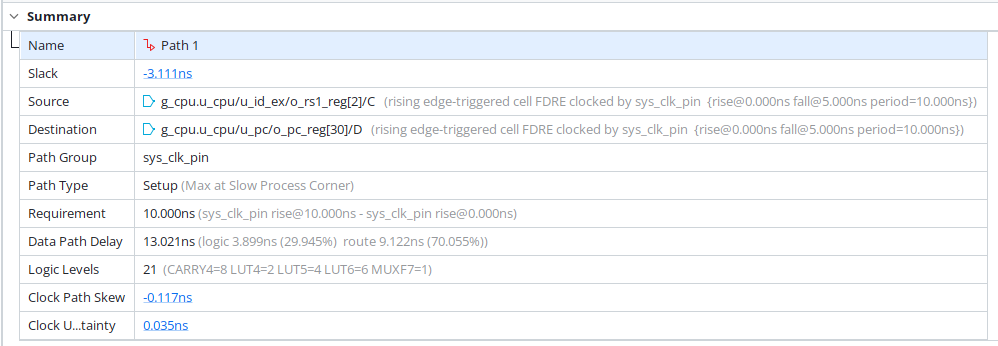
\includegraphics[width=\textwidth]{path1-summary.png}
  \caption{Resumen del camino crítico a 100~MHz (Path~1).}
  \label{fig:path100}
\end{figure}

El detalle celda por celda (anexo~\ref{anexo:camino}) muestra el recorrido,
que es el esperado para esta arquitectura, porque todo ocurre en un solo ciclo
de EX:
\begin{enumerate}[nosep]
  \item el operando sale de ID/EX y pasa por el \textbf{multiplexor de
        forwarding} (la señal \texttt{forward\_a} tiene un fan-out de 64,
        porque controla los 32~bits de dos multiplexores);
  \item atraviesa la \textbf{ALU}, que resta los operandos para comparar los
        de \texttt{beq}/\texttt{bne};
  \item la \textbf{decisión del salto} (fan-out de 37) selecciona el destino;
  \item termina en una cadena de 8 bloques \textbf{CARRY4} (un sumador de
        32~bits) que calcula el \textbf{próximo PC}.
\end{enumerate}

La frecuencia máxima estimada es
$f_{\max} \approx 1/(10~\text{ns} + 3{,}111~\text{ns}) \approx 76$~MHz. Siete de
cada diez nanosegundos del camino son de ruteo, no de lógica.

\subsubsection{Frecuencia final: 62,5~MHz}

Para bajar la frecuencia sin intervenir el clock se usó un MMCM, configurado
con el Clocking Wizard (\texttt{clk\_wiz\_0}). Se eligió \textbf{62,5~MHz},
un 18\% por debajo del máximo estimado, por dos razones:
\begin{itemize}[nosep]
  \item deja margen frente al máximo de $\approx 76$~MHz, que es solo una
        estimación y cambia entre corridas de implementación;
  \item se obtiene con divisores enteros
        ($100~\text{MHz} \cdot 10 / 1 = 1\,000~\text{MHz}$ en el VCO, dividido
        por 16), lo que da un clock de salida exacto y con menos jitter que una
        configuración fraccionaria.
\end{itemize}

\begin{figure}[H]
  \centering
  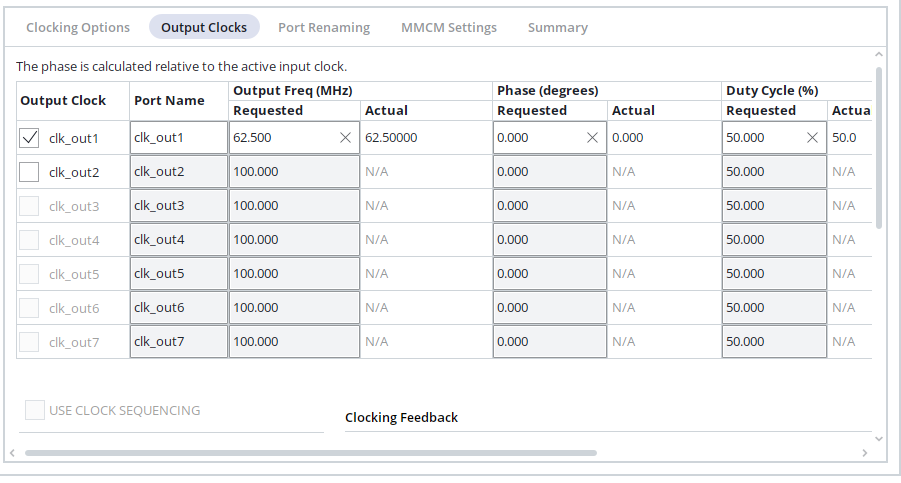
\includegraphics[width=0.85\textwidth]{clk-wiz-output.png}
  \caption{Clocking Wizard: una sola salida, \texttt{clk\_out1}, de
  62,5~MHz pedidos y 62,5~MHz obtenidos, fase 0 y ciclo de trabajo 50\%.}
  \label{fig:clkwiz}
\end{figure}

\begin{figure}[H]
  \centering
  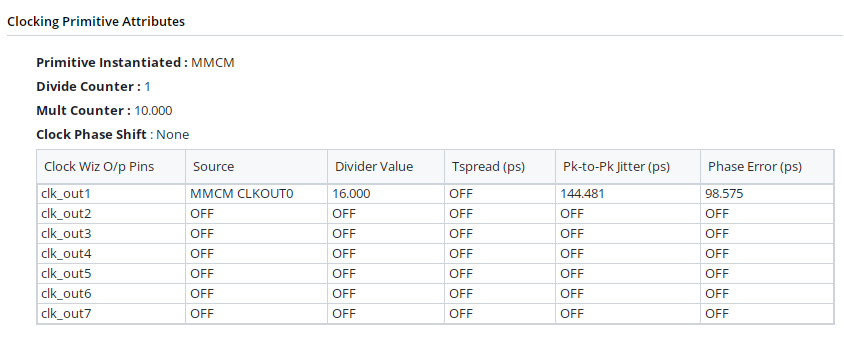
\includegraphics[width=0.85\textwidth]{summary-62-5MHz.png}
  \caption{Atributos del MMCM generado: $D = 1$, $M = 10$, $O = 16$, jitter
  pico a pico de 144,481~ps y error de fase de 98,575~ps.}
  \label{fig:mmcm}
\end{figure}

\begin{table}[H]
\centering
\small
\begin{tabular}{@{}ll@{}}
\toprule
Parámetro del MMCM & Valor \\
\midrule
Entrada & 100~MHz (pin W5) \\
$M$ / $D$ / $O$ & 10 / 1 / 16 \\
$f_{\text{VCO}} = f_{\text{in}} \cdot M / D$ & 1\,000~MHz \\
$f_{\text{out}} = f_{\text{VCO}} / O$ & 62,5~MHz (período de 16~ns) \\
Jitter pico a pico / error de fase & 144,481~ps / 98,575~ps \\
\bottomrule
\end{tabular}
\caption{Configuración del Clocking Wizard.}
\end{table}

A 62,5~MHz la implementación \textbf{cumple todas las restricciones de timing}
(figura~\ref{fig:wns62}):

\begin{figure}[H]
  \centering
  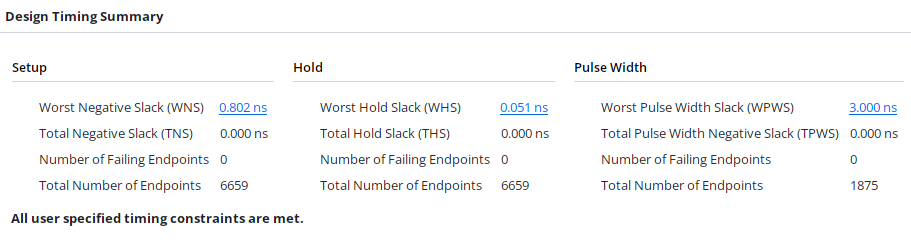
\includegraphics[width=\textwidth]{new-wns.png}
  \caption{Resumen de timing a 62,5~MHz: setup, hold y ancho de pulso cumplen,
  sin endpoints fallando.}
  \label{fig:wns62}
\end{figure}

\begin{table}[H]
\centering
\small
\begin{tabular}{@{}lL{10cm}@{}}
\toprule
Medida & Valor a 62,5~MHz \\
\midrule
WNS / TNS & $+0{,}802$~ns / 0~ns (0 de 6\,659 endpoints fallando) \\
WHS / THS & $+0{,}051$~ns / 0~ns \\
WPWS & $+3{,}000$~ns \\
Camino crítico & \texttt{u\_ex\_mem/o\_rd\_reg[0]} $\rightarrow$ \texttt{u\_id\_ex/o\_rs1\_data\_reg[13]} (entrada R) \\
Niveles de lógica & 17 (4 CARRY4, 1 LUT2, 1 LUT3, 2 LUT5, 8 LUT6, 1 MUXF7) \\
Retardo del camino & 14,494~ns: 3,719~ns de lógica (26\%) y 10,775~ns de ruteo (74\%) \\
Skew / incertidumbre del clock & $-0{,}099$~ns / 0,080~ns \\
\bottomrule
\end{tabular}
\caption{Resultado de timing a la frecuencia final, con el MMCM.}
\end{table}

\begin{figure}[H]
  \centering
  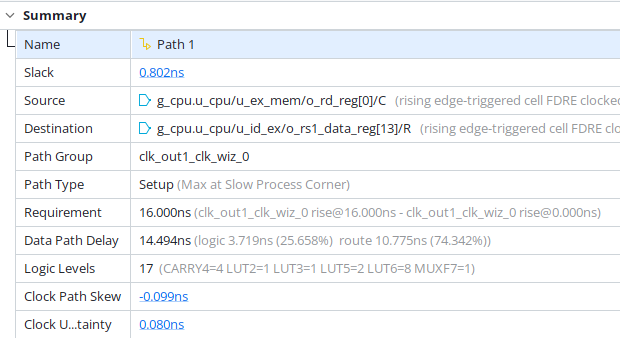
\includegraphics[width=0.75\textwidth]{skew.png}
  \caption{Camino crítico a 62,5~MHz: slack de $+0{,}802$~ns y skew del clock
  de $-0{,}099$~ns.}
  \label{fig:path62}
\end{figure}

El camino crítico cambia de extremo pero es de la misma naturaleza. Parte del
\texttt{rd} guardado en EX/MEM, que la \texttt{forwarding\_unit} compara con los
registros fuente de la instrucción en EX; de ahí pasa por el multiplexor de
forwarding, la ALU y la decisión del salto, y termina en la entrada de reset
sincrónico (R) de ID/EX, que es el \textbf{flush} cuando el salto se toma. Es
decir, sigue siendo ``forwarding $\rightarrow$ ALU $\rightarrow$ decisión del
salto'' en un solo ciclo. Cuando el diseño ya cumple, Vivado deja de optimizar
ese camino, por eso su retardo no es comparable directamente con el de la
corrida a 100~MHz. En ambas corridas el ruteo es más del 70\% del retardo.

Todo el diseño usa la salida del MMCM, y su señal \texttt{locked} mantiene el
sistema en reset hasta que el clock es estable. El parámetro
\texttt{CLK\_FREQ} del top debe valer 62\,500\,000, porque la UART calcula su
divisor a partir de él: si no coincidiera con el clock real, la velocidad de
transmisión sería incorrecta.

\textbf{Restricción del clock y reporte de metodología.} Además del análisis
de timing, Vivado revisa las restricciones con \texttt{report\_methodology}. En
una primera versión, \texttt{top.xdc} definía el clock del pin con la opción
\texttt{-add}:

\begin{center}
\footnotesize\texttt{create\_clock -add -name sys\_clk\_pin -period 10.00 -waveform \{0 5\} [get\_ports i\_clk]}
\end{center}

\noindent y el reporte encontraba cuatro problemas:

\begin{table}[H]
\centering
\small
\begin{tabular}{@{}llL{8.4cm}c@{}}
\toprule
Regla & Severidad & Descripción & Casos \\
\midrule
TIMING-6 & Critical Warning & \texttt{clk\_out1\_clk\_wiz\_0} y \texttt{clk\_out1\_clk\_wiz\_0\_1} se analizan juntos pero no tienen un clock primario común & 2 \\
TIMING-56 & Warning & dos clocks generados en el mismo pin del MMCM (\texttt{CLKOUT0} y \texttt{CLKFBOUT}) sin declararse excluyentes & 2 \\
\bottomrule
\end{tabular}
\caption{\texttt{report\_methodology} con \texttt{create\_clock -add}.}
\end{table}

La causa es que el Clocking Wizard trae su propio archivo de restricciones,
que ya define un clock de 10~ns en su entrada, conectada al puerto
\texttt{i\_clk}. Con \texttt{-add}, el \texttt{create\_clock} de
\texttt{top.xdc} no reemplaza esa definición sino que \emph{agrega} un segundo
clock primario en el mismo pin. Vivado deriva entonces dos copias de cada salida
del MMCM (\texttt{clk\_out1\_clk\_wiz\_0} y \texttt{clk\_out1\_clk\_wiz\_0\_1}, y lo
mismo con la realimentación \texttt{clkfbout}). Como las dos copias llegan a los
mismos flip-flops, analiza caminos entre ellas, pero sin un origen común no
puede saber su relación de fase: por eso advierte que el diseño ``podría fallar
en hardware'' (TIMING-6) y que hay clocks duplicados en un mismo pin
(TIMING-56). En realidad es un único clock físico definido dos veces. Quitar
\texttt{-add} elimina los cuatro avisos, porque la definición de
\texttt{top.xdc} pasa a \emph{reemplazar} a la del IP, pero Vivado advierte
entonces que se pisa una definición anterior (\texttt{Constraints 18-1055}) y
se pierde el jitter de entrada que el IP declara junto con su clock. La
solución final fue \textbf{no redeclarar el clock en \texttt{top.xdc}}: el
\texttt{create\_clock} quedó comentado, el clock de 10~ns lo define únicamente
el Clocking Wizard y Vivado deriva de él una sola copia de cada salida del MMCM.
Declarar los clocks como excluyentes con \texttt{set\_clock\_groups} también
habría silenciado los avisos, pero dejaba dos definiciones del mismo clock
físico. (En el intento a 100~MHz, sin el MMCM, sí hacía falta el
\texttt{create\_clock} propio, porque no había IP que lo definiera.)

\textbf{Skew.} Todo camino tiene un skew entre su flip-flop de origen y el de
destino. En el camino crítico vale $-0{,}099$~ns: es pequeño porque hay un único
clock, que sale del MMCM y se distribuye por la red global dedicada (BUFG), sin
pasar por lógica. Por eso no compromete el diseño.

Vivado calcula el skew como la diferencia entre el instante en que el clock
llega al flip-flop de destino y el instante en que llega al de origen, y lo
incluye en el slack. En el intento a 100~MHz (anexo~\ref{anexo:camino}) se ve el
cálculo completo: el flanco llega al origen a los 5,082~ns (1,458~ns del IBUF,
1,967~ns hasta el BUFG, 0,096~ns del BUFG y 1,561~ns de la red global) y al
destino a los 4,777~ns después de su flanco; sumando 0,188~ns de
\emph{clock pessimism removal}, el skew es
$4{,}777 + 0{,}188 - 5{,}082 = -0{,}117$~ns. Un skew negativo resta tiempo al
camino de setup, pero en ambos casos es del orden del 1\% del período.

\subsection{Recursos}

El diseño completo ocupa una fracción chica del XC7A35T
(figura~\ref{fig:util}). No usa Block RAM: las memorias de programa y de datos
se infieren como RAM distribuida (``LUT as Memory'' en la
figura~\ref{fig:jerarquia}), como se buscaba.

\begin{table}[H]
\centering
\small
\begin{tabular}{@{}lrrr@{}}
\toprule
Recurso & Usados & Disponibles & Uso \\
\midrule
LUT & 2\,449 & 20\,800 & 11,8\% \\
\quad como lógica & 2\,241 & 20\,800 & 10,8\% \\
\quad como RAM distribuida & 208 & 9\,600 & 2,2\% \\
Flip-flops & 1\,629 & 41\,600 & 3,9\% \\
Slices & 1\,148 & 8\,150 & 14,1\% \\
MUXF7 / MUXF8 & 435 / 165 & 16\,300 / 8\,150 & 2,7\% / 2,0\% \\
Block RAM & 0 & 50 & 0\% \\
IOB & 12 & 106 & 11,3\% \\
BUFG & 2 & 32 & 6,3\% \\
MMCM & 1 & 5 & 20\% \\
\bottomrule
\end{tabular}
\caption{Utilización después de la implementación, a 62,5~MHz.}
\end{table}

\begin{figure}[htbp]
  \centering
  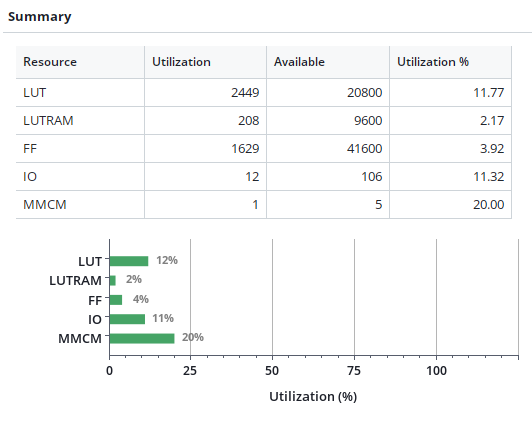
\includegraphics[width=0.5\textwidth]{resource-utilization.png}
  \caption{Utilización post-implementación.}
  \label{fig:util}
\end{figure}

\begin{figure}[htbp]
  \centering
  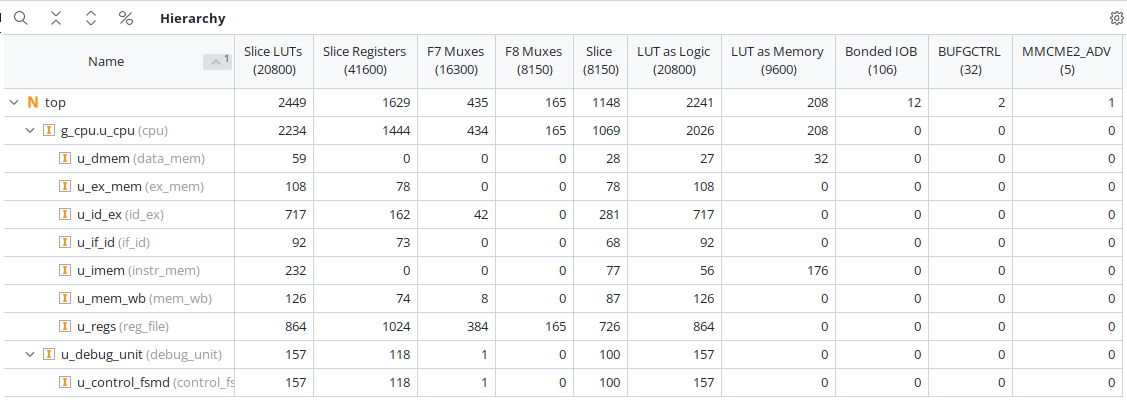
\includegraphics[width=\textwidth]{resource-hierarchy.png}
  \caption{Utilización por módulo.}
  \label{fig:jerarquia}
\end{figure}

La distribución por módulo (figura~\ref{fig:jerarquia}) muestra que:
\begin{itemize}[nosep]
  \item el \textbf{procesador} usa el 91\% de las LUT (2\,234) y el 89\% de los
        flip-flops (1\,444);
  \item el \textbf{banco de registros} es el bloque más grande: 1\,024
        flip-flops ($32 \times 32$~bits) y 864 LUT, más todos los MUXF8, que
        forman los multiplexores de lectura de 32 a 1 de sus tres puertos
        (\texttt{rs1}, \texttt{rs2} y el de debug);
  \item \texttt{u\_id\_ex} reúne 717 LUT porque, al optimizar, Vivado agrupa
        bajo ese nombre la lógica de EX que se alimenta de él: forwarding, ALU
        y saltos;
  \item la \textbf{memoria de programa} usa 176 LUT como RAM (256 palabras) y
        la \textbf{de datos} 32 (32 palabras);
  \item la \textbf{Debug Unit} es chica: 157 LUT y 118 flip-flops, todos en
        \texttt{control\_fsmd}; el volcado ``al vuelo'' no necesita buffer.
\end{itemize}

\subsection{Prueba con la PC}

El sistema se probó en la placa a 62,5~MHz, conectado a la PC por USB, con el
depurador gráfico y con \texttt{uart\_test.py}, siguiendo el procedimiento de
\texttt{docs/CHECKLIST\_placa.md}: carga de programas, ejecución continua y
paso a paso, interrupción de un programa sin fin, reprogramación y reset.

% ============================================================
\section{Respuestas a las preguntas de la consigna}
% ============================================================

\subsection{Reprogramación}

\begin{table}[H]
\centering
\small
\begin{tabular}{@{}L{3.6cm}L{4.4cm}L{6.4cm}@{}}
\toprule
Pregunta & Respuesta & Justificación \\
\midrule
¿Es necesario vaciar la memoria de datos? & No. Es RAM y el reset no la borra. & Una RAM no se borra con un reset; borrarla exigiría implementarla con flip-flops. Cada programa inicializa los datos que usa, como en cualquier computadora. \\
¿Y los registros? & Sí: el reset que hace \cmd{L} los pone en cero. & Son estado del procesador: el programa nuevo no depende del anterior. \\
¿Se necesita vaciar el pipeline? & Sí: el reset deja los cuatro registros de pipeline como burbujas y el PC en cero. & Si no, instrucciones del programa anterior terminarían de ejecutarse. \\
¿Y la memoria de programa? & No con el reset; sí con la carga: CLEAR escribe HALT en lo que el programa no usa. & El reset la conserva para poder repetir el programa con \cmd{X}; el CLEAR evita restos del programa anterior. \\
\bottomrule
\end{tabular}
\caption{Qué se vacía al reprogramar.}
\end{table}

\subsection{¿Qué sucede si no hay instrucción de parada?}

No puede ocurrir del todo: después de un \cmd{L} todas las palabras que el
programa no usa contienen HALT, y la palabra 255 siempre es HALT. Un programa
sin HALT termina en el primer HALT de relleno; incluso uno que ocupa las 256
palabras, porque la última se reemplaza por HALT (\texttt{NOPx256}: 255 NOP más
el HALT, $255 + 4 = 259$ ciclos). Lo que sí puede ocurrir es un
\emph{loop infinito}: \cmd{R} no termina y la Debug Unit lo corta con \cmd{I},
devolviendo el estado con el bit de interrumpido (0x02). Un salto fuera de la
memoria de programa o desalineado detiene el procesador con error (0x05).

\begin{figure}[H]
  \centering
  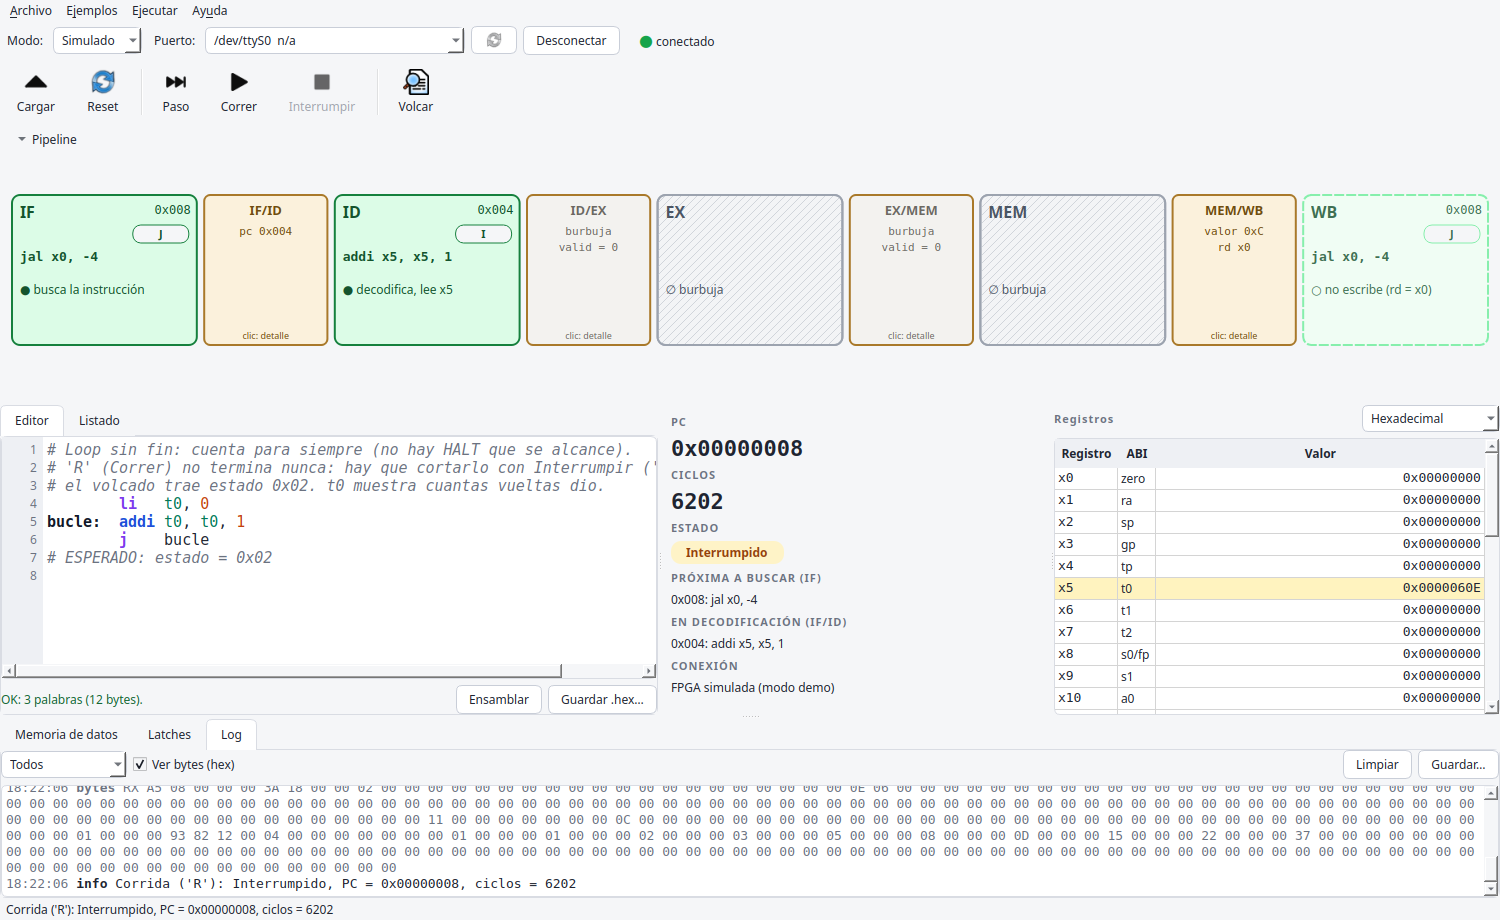
\includegraphics[width=\textwidth]{depurador_interrumpido_log.png}
  \caption{Loop sin fin cortado con \cmd{I}: estado ``Interrumpido'' después de
  6\,202 ciclos, \texttt{t0} con la cantidad de vueltas y, abajo, los bytes del
  volcado en el registro de eventos.}
  \label{fig:interrumpido}
\end{figure}

\subsection{Camino crítico, skew y frecuencia}

Respondidas en la sección~\ref{sec:timing}:
\begin{itemize}[nosep]
  \item \textbf{Camino crítico:} forwarding $\rightarrow$ ALU $\rightarrow$
        decisión del salto $\rightarrow$ próximo PC (o flush de ID/EX), todo en
        el ciclo de EX. A 100~MHz tiene 21 niveles de lógica y 13,021~ns, con un
        70\% de ruteo.
  \item \textbf{Skew:} $-0{,}099$~ns en el camino crítico a 62,5~MHz. Es
        pequeño porque hay un único clock, distribuido desde el MMCM por la red
        global (BUFG) sin pasar por lógica.
  \item \textbf{Frecuencia:} 100~MHz no cumple (WNS $= -3{,}111$~ns,
        $f_{\max} \approx 76$~MHz). El diseño trabaja a \textbf{62,5~MHz},
        generados con el Clocking Wizard, con WNS $= +0{,}802$~ns y WHS
        $= +0{,}051$~ns.
\end{itemize}

% ============================================================
\section{Conclusiones}
% ============================================================

\begin{itemize}
  \item \textbf{Rendimiento del pipeline.} El número de ciclos sigue exactamente
  $N + 4 + \text{stalls} + 2 \cdot \text{saltos tomados}$, lo que se verificó en
  todos los programas. El forwarding elimina las esperas en todas las
  dependencias salvo el load-use (1~ciclo), y la penalidad dominante es la de
  los saltos tomados: en Fibonacci, 62 de los 66 ciclos por encima de una
  instrucción por ciclo vienen de los 31 saltos, y el CPI resulta 1,34. Resolver
  los saltos en ID bajaría la penalidad a 1~ciclo (CPI $\approx 1{,}18$ en ese
  programa), a costa de un comparador y forwarding hacia ID.

  \item \textbf{Frecuencia.} La decisión de resolver los saltos en EX con los
  operandos adelantados concentra en un solo ciclo el forwarding, la ALU y la
  selección del próximo PC: es el camino crítico (21 niveles de lógica,
  13,02~ns a 100~MHz) y limita la frecuencia a $\approx 76$~MHz, por lo que
  los 100~MHz del oscilador no cumplen timing (WNS $= -3{,}111$~ns). El diseño
  trabaja a 62,5~MHz con un MMCM de divisores enteros ($M = 10$, $D = 1$,
  $O = 16$), con WNS $= +0{,}802$~ns. Más del 70\% del retardo del camino es
  ruteo, agravado por señales de gran fan-out como la selección de forwarding
  (64) y la decisión del salto (37). Comparar los operandos del salto con un
  comparador dedicado en lugar de la resta de la ALU, o registrar la decisión
  del salto antes de usarla en el PC y en el flush, acortaría ese camino y
  permitiría subir la frecuencia.

  \item \textbf{Recursos.} El sistema completo usa el 11,8\% de las LUT y el
  3,9\% de los flip-flops del XC7A35T, sin Block RAM. El banco de registros es
  el bloque más costoso (1\,024 flip-flops y 864 LUT), por sus tres puertos de
  lectura asincrónica, mientras que la Debug Unit ocupa solo 157 LUT gracias al
  volcado generado al vuelo.

  \item \textbf{Clock enable.} Controlar la ejecución con un clock enable, y no
  intervenir el clock, permitió implementar el modo paso a paso, la pausa y la
  parada con un único clock y sin cruces de dominio, y mantuvo válido el
  análisis estático de timing.

  \item \textbf{Memorias.} La RAM distribuida con lectura asincrónica mantuvo un
  pipeline de cinco etapas sin ciclos extra de latencia en IF y en MEM, y
  permitió armar el volcado al vuelo. El tamaño de la memoria de datos (32
  palabras) se igualó a lo que muestra el volcado, de modo que toda la memoria
  es observable.

  \item \textbf{Observabilidad.} Exponer los 480~bits de los registros de
  pipeline, alineados a palabras, junto con un volcado de 326~bytes generado sin
  buffer, hace posible ver cada fenómeno del pipeline ciclo a ciclo. Como los
  registros de pipeline no guardan el PC en EX/MEM y MEM/WB, la instrucción en
  esas etapas debe deducirse; agregar esos dos PC al volcado lo haría directo.

  \item \textbf{Verificación.} Contrastar el RTL contra un modelo de referencia
  independiente y contra cuentas a mano, y medir la calidad de los tests con
  pruebas de mutación (12 de 12 detectadas), permitió encontrar diferencias
  reales en la integración ---la latencia del HALT, \texttt{x0} por debug y el
  tamaño de la memoria de datos--- antes de llevar el diseño a la placa. El
  contrato escrito y el \texttt{cpu\_stub} permitieron desarrollar el
  procesador y la Debug Unit en paralelo e integrarlos con cambios acotados.
\end{itemize}

% ============================================================
\begin{thebibliography}{9}
\bibitem{patterson}
D.~A. Patterson y J.~L. Hennessy, \emph{Computer Organization and Design RISC-V
Edition: The Hardware Software Interface}, 2.ª ed. Morgan Kaufmann, 2020.

\bibitem{riscv}
RISC-V International, \emph{The RISC-V Instruction Set Manual, Volume I:
Unprivileged ISA}, \url{https://riscv.org/specifications/}.

\bibitem{chu}
P.~P. Chu, \emph{FPGA Prototyping by Verilog Examples: Xilinx Spartan-3 Version}.
Wiley, 2008.

\bibitem{ug472}
Xilinx, \emph{7 Series FPGAs Clocking Resources User Guide} (UG472).

\bibitem{pg065}
Xilinx, \emph{Clocking Wizard LogiCORE IP Product Guide} (PG065).

\bibitem{basys3}
Digilent, \emph{Basys 3 FPGA Board Reference Manual}, 2016.

\bibitem{xdc}
Digilent, \emph{Basys-3-Master.xdc}, repositorio \texttt{digilent-xdc},
\url{https://github.com/Digilent/digilent-xdc}.

\bibitem{catedra}
Cátedra de Arquitectura de Computadoras, \emph{Trabajo Final: Pipeline
Procesador (RISC-V)}, FCEFyN, UNC, 2026.
\end{thebibliography}

% ============================================================
\appendix
\section{Detalle del camino crítico a 100~MHz}
\label{anexo:camino}
% ============================================================

Reporte de Vivado del camino crítico del intento a 100~MHz
(sección~\ref{sec:timing100}), de \texttt{u\_id\_ex/o\_rs1\_reg[2]} a
\texttt{u\_pc/o\_pc\_reg[30]}. Las figuras~\ref{fig:dp1} a~\ref{fig:dp3} muestran
el camino de datos celda por celda: la columna \emph{Incr} es el retardo de cada
celda o net y \emph{Path} el tiempo acumulado desde el flanco del clock. Las
figuras~\ref{fig:clk-src} y~\ref{fig:clk-dst} muestran cómo llega el clock al
flip-flop de origen y al de destino, de donde sale el skew.

\begin{figure}[H]
  \centering
  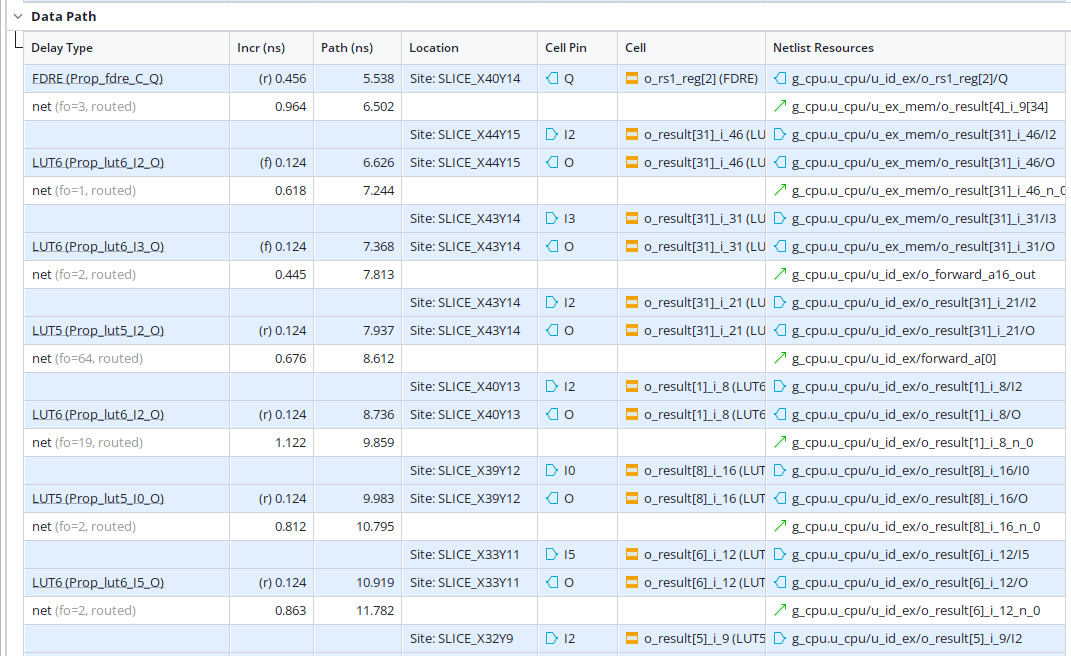
\includegraphics[width=\textwidth]{paht1-data-path1.png}
  \caption{Camino de datos (1/3): de ID/EX, por el multiplexor de forwarding
  (\texttt{forward\_a}, fan-out 64), hacia la ALU.}
  \label{fig:dp1}
\end{figure}

\begin{figure}[H]
  \centering
  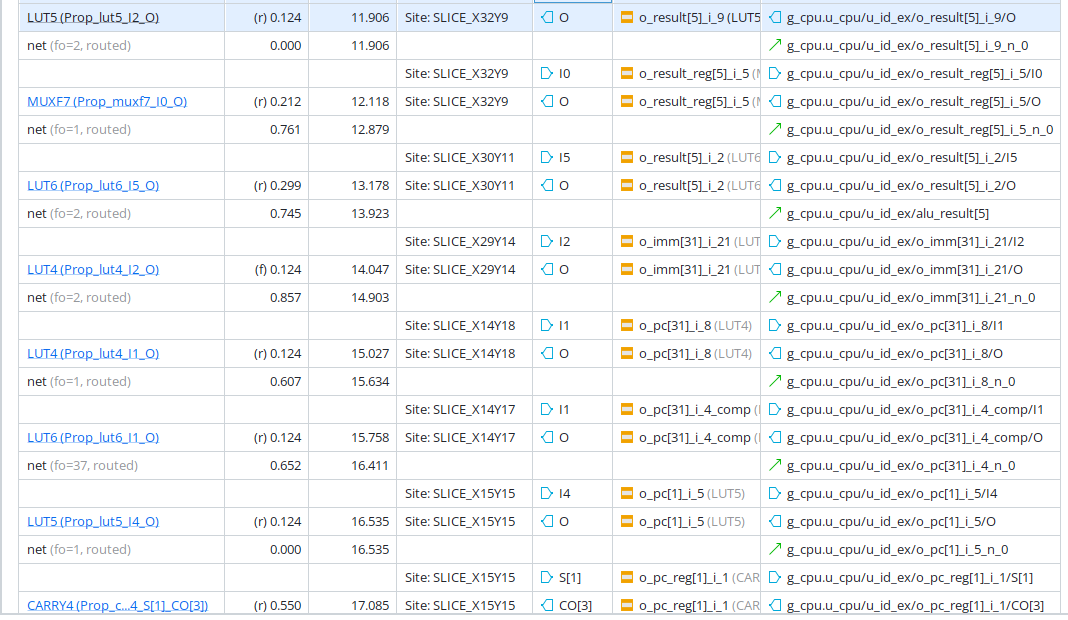
\includegraphics[width=\textwidth]{path1-data-path2.png}
  \caption{Camino de datos (2/3): resultado de la ALU, decisión del salto
  (fan-out 37) y entrada a la cadena de acarreo.}
  \label{fig:dp2}
\end{figure}

\begin{figure}[H]
  \centering
  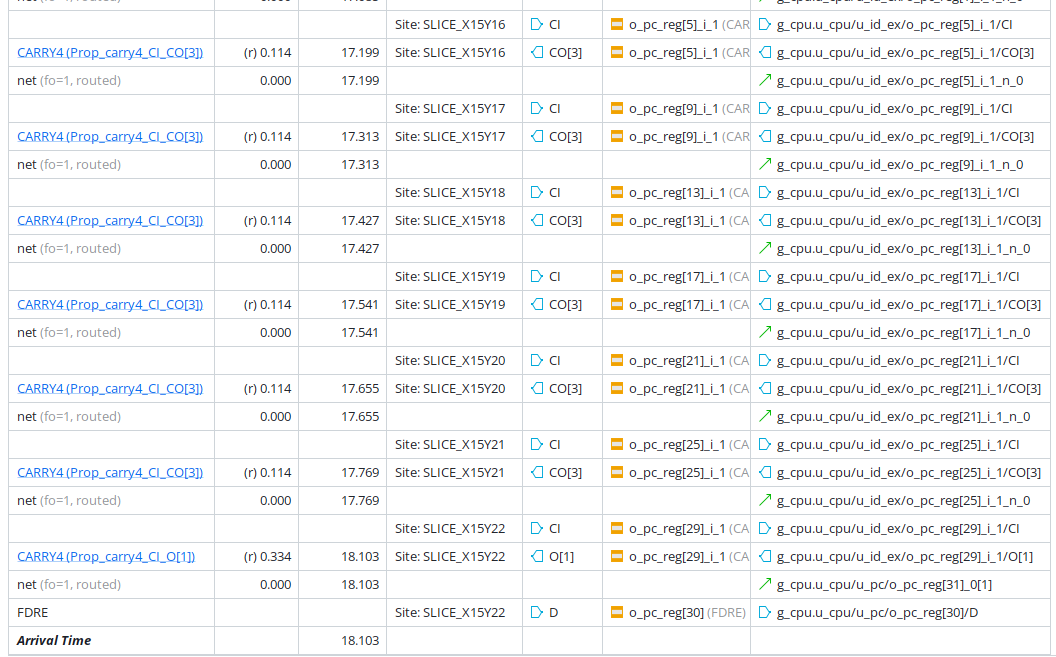
\includegraphics[width=\textwidth]{pah1-data-path3.png}
  \caption{Camino de datos (3/3): cadena de CARRY4 del sumador del próximo PC
  y llegada a \texttt{o\_pc\_reg[30]} a los 18,103~ns.}
  \label{fig:dp3}
\end{figure}

\begin{figure}[H]
  \centering
  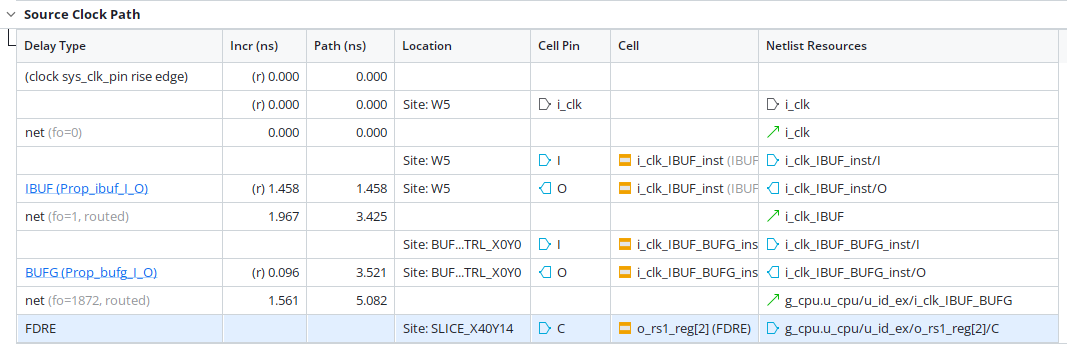
\includegraphics[width=\textwidth]{path1-clock-path.png}
  \caption{Camino del clock al flip-flop de origen: pin W5, IBUF, BUFG y red
  global (fan-out 1\,872); llega a los 5,082~ns.}
  \label{fig:clk-src}
\end{figure}

\begin{figure}[H]
  \centering
  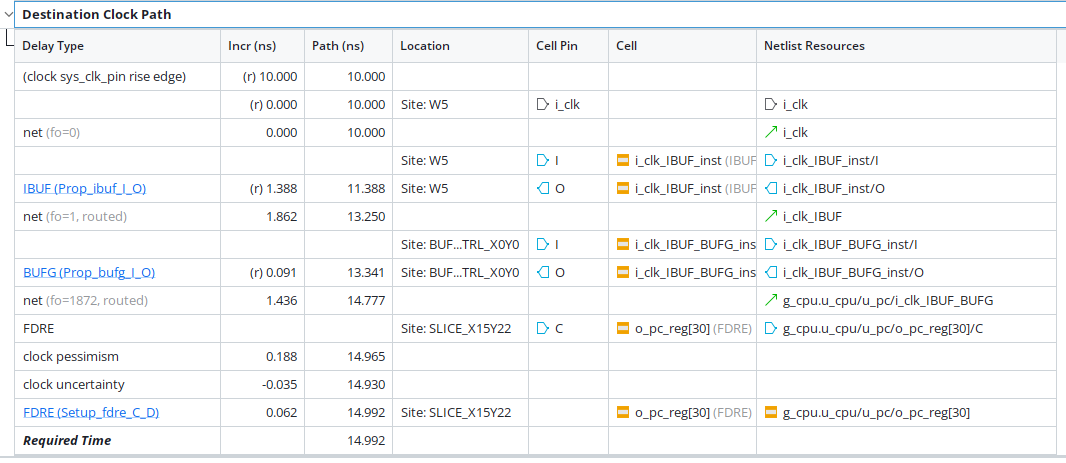
\includegraphics[width=\textwidth]{path1-destination-clock-path.png}
  \caption{Camino del clock al flip-flop de destino, un período después:
  llega a los 14,777~ns; con el \emph{clock pessimism}, la incertidumbre y el
  setup, el tiempo requerido es 14,992~ns, y el slack resulta
  $14{,}992 - 18{,}103 = -3{,}111$~ns.}
  \label{fig:clk-dst}
\end{figure}

\end{document}
